\documentclass[12pt,a4paper]{report}

\usepackage[margin=1in]{geometry}
\usepackage{graphicx}
\usepackage{booktabs}
\usepackage{array}
\usepackage{longtable}
\usepackage{amsmath}
\usepackage{amssymb}
\usepackage{float}
\usepackage{caption}
\usepackage{subcaption}
\usepackage{xcolor}
\usepackage{hyperref}
\usepackage{url}
\usepackage{setspace}
\usepackage{parskip}

\graphicspath{{../results/figures/}}

\hypersetup{
    colorlinks=true,
    linkcolor=blue,
    citecolor=blue,
    urlcolor=blue
}

\setlength{\parskip}{0.6em}
\setlength{\parindent}{0pt}

\title{\textbf{Comparative Topological Analysis of Biological Neural Networks Using Canonical Complex Network Models}\\[1em]
\large A Graph-Theoretic Study of the \textit{Caenorhabditis elegans} Connectome}
\author{Complex Systems Course Project}
\date{May 2026}

\begin{document}

\hypersetup{pageanchor=false}
\pagenumbering{roman}
\maketitle

\begin{abstract}
Understanding how the brain is wired — not just how individual neurons work — is one of the central challenges in modern neuroscience and complex systems science. At the scale of an entire organism, the \textit{Caenorhabditis elegans} nervous system offers a unique window into this problem: it is the only animal for which a complete wiring diagram, or connectome, has been reconstructed at the level of every synapse. This project uses that connectome as an empirical test case to ask a focused question from network science: which canonical class of synthetic graph model most faithfully captures the topological organization of a real biological neural network?

Using the OpenWorm ConnectomeToolbox dataset derived from the electron microscopy reconstructions of White et al.~\cite{white1986structure}, we construct an undirected graph of 309 nodes and 2{,}511 edges representing synaptic connections across the \textit{C. elegans} nervous system. We then generate four families of synthetic comparison networks — Erd\H{o}s--R\'{e}nyi random graphs, regular ring lattices, Watts--Strogatz small-world graphs, and Barab\'{a}si--Albert scale-free graphs — each matched in size and approximate density to the biological network. For each graph we compute a broad suite of topological metrics encompassing clustering, path length, degree heterogeneity, modularity, assortativity, and global efficiency. We further examine robustness under two distinct node-removal strategies. The comparison is formalized through a normalized multi-metric distance score.

The biological connectome exhibits a rich topology that no single canonical model reproduces well: average clustering of 0.351, average shortest path length of 2.665, a degree variance of 180 driven by a small number of high-degree command interneurons, clear modular organization into four communities, and a disassortative mixing pattern in which hubs preferentially connect to low-degree neurons. Under the normalized distance ranking, the Barab\'{a}si--Albert scale-free model is closest to the empirical graph (distance 0.300), followed by Watts--Strogatz (0.346), Erd\H{o}s--R\'{e}nyi (0.454), and the regular lattice (0.982). However, the strongest result is that the \textit{C. elegans} connectome is not well approximated by any single model: it combines hub-driven degree heterogeneity characteristic of scale-free graphs with clustering and path efficiency characteristic of small-world graphs, and adds modularity and disassortativity that neither canonical family captures fully. The evidence points firmly toward a hybrid complex-network interpretation shaped by the biological demands of efficient sensing, integration, and motor coordination in a compact nervous system.
\end{abstract}

\tableofcontents
\listoffigures
\listoftables
\clearpage
\hypersetup{pageanchor=true}
\pagenumbering{arabic}

%% ============================================================
\chapter{Introduction}
%% ============================================================

\section{The Topology of Thought}

The brain is, in the most literal sense, a network. Individual neurons are meaningless in isolation: what they do depends entirely on which other neurons they are connected to, and how. This insight has a long history in neuroscience, but only in the past three decades has it become possible to study neuronal connectivity at the level of every synapse in an entire organism. The result is the field of connectomics — the large-scale, systematic mapping of neural wiring diagrams.

At the same time, network science has developed a powerful formal vocabulary for characterizing the structure of complex systems. Graph theory provides metrics that capture qualitatively different aspects of how a network is organized: how clustered its neighborhoods are, how efficiently signals can travel from one node to another, whether some nodes serve as disproportionate hubs, and whether the network decomposes into semi-independent communities. Applied to biological data, these tools allow us to ask whether the nervous system's architecture resembles any of the idealized network families that theorists have studied, and if so, what that resemblance implies about the principles governing neural organization.

This project sits at the intersection of those two programs. We apply the language and metrics of complex network science to the most completely characterized nervous system available — that of the nematode \textit{Caenorhabditis elegans} — and ask a concrete comparative question:

\begin{quote}
\textit{Among the canonical synthetic network models of complex systems theory — random, lattice, small-world, and scale-free — which class of graph best approximates the topology of the \textit{C. elegans} connectome?}
\end{quote}

This question matters for several reasons. If the nervous system resembles a random graph, it suggests that its connectivity is shaped primarily by developmental constraints or physical proximity rather than functional organization. If it resembles a small-world graph, it implies that evolution has struck a balance between local processing efficiency and global integration speed. If it resembles a scale-free network, it suggests that certain neurons play a disproportionate integrative role and that the system's robustness profile is asymmetric — resilient to random damage but fragile to targeted attack on its hubs. In practice, real biological networks may blend features from multiple canonical classes, and identifying which features are borrowed from which model — and which features are genuinely novel — is itself a meaningful scientific contribution.

\section{Why \textit{C. elegans}?}

The choice of \textit{C. elegans} as the empirical system is deliberate and not incidental. This microscopic soil nematode has exactly 302 neurons in its hermaphrodite form, and the complete connectivity of its nervous system was mapped by electron microscopy nearly four decades ago by White, Southgate, Thomson, and Brenner \cite{white1986structure}. That original 1986 reconstruction remains a foundational achievement: it was the first and, for a long time, the only complete wiring diagram of any animal nervous system.

What makes the \textit{C. elegans} connectome scientifically attractive beyond its historical importance is the combination of completeness and tractability. With 302 neurons and a few thousand synapses, it is small enough to analyze comprehensively with graph-theoretic tools, yet complex enough to support behavioral repertoires including locomotion, chemosensation, thermosensation, mechanosensation, and reproduction. Many of the identified circuit motifs — such as the command interneurons that coordinate forward and backward movement — have direct behavioral correlates that can be tested experimentally. This means that the abstract network metrics we compute are not just mathematical curiosities; they can, in principle, be connected back to what the animal actually does.

The dataset used in this project is the OpenWorm ConnectomeToolbox version of the White 1986 whole-animal connectivity table \cite{openwormtoolbox}, which provides a digitized and curated edge list encoding presynaptic neuron, postsynaptic target, connection type (chemical synapse or gap junction), and synapse count. This data represents the most widely used and biologically grounded version of the \textit{C. elegans} connectome for computational studies.

\section{Scope and Contribution}

This project performs a systematic, reproducible, end-to-end comparison of the \textit{C. elegans} connectome against four canonical synthetic network models. The comparison uses a multi-metric framework that evaluates clustering, path length, density, degree heterogeneity, modularity, assortativity, and global efficiency simultaneously. It extends the metric analysis with robustness experiments under random and targeted node removal, which probe properties that scalar metrics cannot capture directly.

The goal is not to claim that the \textit{C. elegans} nervous system \textit{is} a scale-free or small-world graph in some definitive categorical sense. The goal is to produce a quantified, multi-dimensional characterization of how closely each canonical family approximates the empirical topology, and to reason about what the pattern of similarities and differences implies for how we should think about biological neural network organization.


%% ============================================================
\chapter{Background}
%% ============================================================

\section{Networks as a Scientific Language}

A graph $G = (V, E)$ consists of a set of vertices $V$ and a set of edges $E \subseteq V \times V$. This deceptively simple abstraction is powerful precisely because it strips away the particular details of any system and retains only the pattern of connections. When applied to a nervous system, nodes represent neurons (or other biological units such as muscles) and edges represent synaptic or electrical connections between them. The resulting graph can then be analyzed using the full toolkit of graph theory and network science.

The value of this abstraction is not that it is complete — it discards directionality, synaptic strength, neurotransmitter identity, spatial geometry, and countless other biological details — but that it is \textit{tractable}. Graph-theoretic metrics provide principled summaries of structural organization that can be computed consistently, compared across systems, and connected to theory. And critically, they have proven to be far from trivial: across diverse biological, social, and technological systems, the topology of networks turns out to encode information about how those systems function, how they were built, and how robust they are to perturbation~\cite{newman2010networks}.

\section{Key Topological Metrics and Their Meaning}

Before describing the comparison models, it is worth building up an intuition for the metrics used in this analysis. Each metric captures a different structural property, and understanding what each one measures — and what it cannot measure — is essential for interpreting the results.

\paragraph{Clustering coefficient.} The local clustering coefficient of a node $v$ with degree $k_v$ is the fraction of its $k_v(k_v-1)/2$ possible neighbor pairs that are actually connected. A high clustering coefficient means that a node's neighbors tend to be connected to one another — they form a tightly-knit local group, or clique. The average clustering coefficient $\langle C \rangle$ summarizes this tendency across the whole graph. In a neural context, high clustering indicates the presence of local processing circuits: groups of neurons that are densely interconnected and likely share a functional role.

\paragraph{Average shortest path length.} The shortest path between two nodes is the minimum number of edges that must be traversed to get from one to the other. The average shortest path length $\langle L \rangle$ averages this quantity over all pairs of connected nodes. Short path lengths mean that signals can reach any part of the network quickly, supporting rapid global integration. Long path lengths indicate that signals must pass through many relay points, which can introduce delays and reduce the efficiency of information transfer across distant regions.

\paragraph{Global efficiency.} Global efficiency, defined by Latora and Marchiori \cite{latora2001efficient} as $E_{\text{glob}} = \frac{1}{N(N-1)} \sum_{i \neq j} \frac{1}{d_{ij}}$, where $d_{ij}$ is the shortest path length between nodes $i$ and $j$, provides an alternative measure of integration that handles disconnected graphs gracefully (isolated nodes contribute zero efficiency, whereas the average path length is technically undefined for disconnected graphs). It captures how efficiently the network transmits information on average.

\paragraph{Degree and degree heterogeneity.} The degree $k_v$ of a node is the number of edges incident to it. The average degree $\langle k \rangle$ characterizes overall network density. The variance of the degree distribution is a critical quantity: a graph where all nodes have nearly the same degree is qualitatively different from one where most nodes have low degree and a few have extremely high degree. Degree variance measures this heterogeneity. In biological terms, high-degree nodes (hubs) can serve as integration points where many signals converge, while low-degree nodes may serve more specialized or peripheral roles.

\paragraph{Modularity and community structure.} Many real networks divide naturally into communities — groups of nodes that are more densely connected internally than they are to the rest of the network. Modularity $Q$ quantifies the strength of this community structure relative to a random baseline. A modular nervous system is one where functionally distinct circuits (locomotion, feeding, sensory processing) are reflected in the topology: neurons within a circuit are more connected to each other than to neurons in other circuits.

\paragraph{Degree assortativity.} Assortativity $r$ measures whether high-degree nodes tend to connect to other high-degree nodes (assortative, $r > 0$) or whether they tend to connect to low-degree nodes (disassortative, $r < 0$). Social networks tend to be assortative — popular people befriend popular people. Many biological and technological networks are disassortative — hubs connect to periphery nodes. In neural terms, disassortativity is consistent with a hierarchical architecture where command interneurons integrate signals from many sensory neurons and project to many motor neurons, rather than connecting mainly to each other.

\section{The Four Canonical Network Models}

Network science has identified a small set of idealized graph families that have become standard reference points for understanding real-world networks. We briefly describe each, along with its expected properties and the theoretical ideas that motivate it.

\subsection{Erd\H{o}s--R\'{e}nyi Random Graphs}

The Erd\H{o}s--R\'{e}nyi random graph $G(n, m)$ is constructed by placing exactly $m$ edges uniformly at random among $n$ nodes \cite{erdos1959random}. This model is the natural mathematical baseline: it represents the case where connectivity is governed by chance alone, unconstrained by spatial proximity, functional similarity, or any preferential attachment rule.

Random graphs have well-understood properties. When the graph is sufficiently dense, path lengths are short: the diameter grows approximately as $\log n / \log \langle k \rangle$. However, clustering is low — approximately equal to the edge density $p = m/\binom{n}{2}$ — because there is no tendency for neighbors of a node to be connected to each other. Degree distribution is Poisson-distributed, meaning that most nodes have degree close to the mean and extremely high- or low-degree nodes are exponentially rare.

A random graph that matches the \textit{C. elegans} connectome in node and edge count provides a density-controlled null model. Any metric value observed in the biological graph that departs substantially from the random baseline warrants explanation in terms of non-random organizing principles.

\subsection{Regular Ring Lattices}

A regular ring lattice with $k$-nearest-neighbor connectivity places $n$ nodes in a ring, and connects each node to its $k/2$ nearest neighbors on each side. The result is a maximally local network: every node is connected only to those nodes that are physically adjacent on the ring.

Lattice graphs have strikingly opposite properties from random graphs. Clustering is high — around $3(k-2)/4(k-1)$ for large $k$ — because neighboring nodes share most of their neighbors with each other. However, path lengths are very long, scaling as $n/2k$, because to reach a node on the opposite side of the ring one must traverse many local steps. Degree is perfectly uniform: every node has exactly $k$ connections.

The lattice is useful as a structured baseline representing the extreme of local organization. No real large-scale network is a pure lattice, but the lattice's properties define one end of the spectrum that the Watts--Strogatz model interpolates across.

\subsection{Watts--Strogatz Small-World Networks}

The central observation of Watts and Strogatz~\cite{watts1998collective} was that nature appears to prefer a middle ground between random and lattice organization. Their model starts from a ring lattice and then, for each edge, independently rewires it to a randomly chosen target node with probability $p$. At $p=0$, the graph is a pure lattice. At $p=1$, it is approximately random. At intermediate values of $p$, something remarkable happens: even a small fraction of rewired edges dramatically reduces path lengths (because shortcuts can bridge opposite ends of the ring), while leaving clustering largely intact (because the bulk of edges remain local).

This simultaneous combination of high clustering and short path lengths — the small-world property — has been found empirically in a wide variety of real-world systems: social networks, power grids, the \textit{C. elegans} nervous system itself (in the original Watts--Strogatz paper), gene regulatory networks, and the World Wide Web. For a biological nervous system, small-world organization makes functional sense: local clusters support specialized computation, while long-range shortcuts enable rapid coordination across the whole system.

A key parameter in this analysis is choosing the rewiring probability $p$. Rather than picking $p$ arbitrarily, we systematically sweep across a range of values and select the one that best matches the empirical graph, as described in Section~\ref{sec:ws-sweep}.

\subsection{Barab\'{a}si--Albert Scale-Free Networks}

While the small-world model explained the combination of clustering and short paths, it did not address another striking feature of many real networks: the presence of extraordinarily well-connected hubs. Barab\'{a}si and Albert observed that the degree distributions of networks as diverse as the World Wide Web, citation networks, and protein interactions follow a power law, $P(k) \sim k^{-\gamma}$, meaning that the probability of a node having degree $k$ decays only polynomially rather than exponentially~\cite{barabasi1999emergence}. This ``scale-free'' degree distribution implies that extreme hubs — nodes with degrees far above the mean — are far more common than random graph theory would predict.

The BA model produces such distributions through two mechanisms: \textit{growth} (the network expands by adding one node at a time) and \textit{preferential attachment} (each new node connects to $m$ existing nodes with probability proportional to their current degree). The rich-get-richer dynamic means that early nodes accumulate many connections, becoming the dominant hubs of the mature network.

Scale-free networks have several notable properties beyond the degree distribution. They have short path lengths — information moves efficiently through hubs. They have low clustering — hubs connect to many nodes, but those nodes do not necessarily connect to each other. And they have a distinctive robustness profile: they are highly resilient to random node removal (most removed nodes are low-degree and their loss barely affects connectivity) but fragile to targeted removal of hubs.

\section{Why No Single Model Should Be Expected to Suffice}

A biological nervous system is shaped by forces that no canonical graph model represents. Development imposes spatial and temporal constraints on which connections form. Evolution selects for behavioral efficiency and robustness, favoring circuit topologies that accomplish specific functions rather than those that satisfy any abstract mathematical criterion. Cell type diversity creates structural heterogeneity that is not captured by degree distributions alone. Metabolic costs constrain the total number of synapses a nervous system can maintain.

Given these pressures, the expectation should not be that the \textit{C. elegans} connectome is a perfect example of any canonical model. Rather, the interesting scientific question is: which features of its topology are captured by which model, and what does the pattern of matches and mismatches reveal about the organizing principles of biological neural architecture?


%% ============================================================
\chapter{Dataset}
%% ============================================================

\section{\textit{C. elegans}: A Model Organism for Neural Connectivity}

\textit{Caenorhabditis elegans} is a free-living soil nematode approximately one millimeter in length. Despite its simplicity relative to vertebrates, it has been a central model organism in biology since the 1960s, particularly for studying development, genetics, and neuroscience. Its appeal stems from a combination of practical and scientific properties: it is transparent (allowing direct observation of its anatomy through the microscope), it has a short lifespan, it reproduces quickly, its cell lineage is invariant across individuals, and — most relevantly here — it has a compact and well-characterized nervous system.

The hermaphrodite \textit{C. elegans} has exactly 302 neurons, connected by approximately 7{,}000 chemical synapses and 2{,}000 gap junctions. These neurons mediate a rich behavioral repertoire for such a simple organism: forward and backward locomotion, turning, chemosensation, thermosensation, touch avoidance, and feeding. Many specific neurons have known and well-characterized functional roles. The AVA command interneurons (AVAL and AVAR), for instance, are essential for backward locomotion — ablating them prevents backward movement. The AVB interneurons (AVBL and AVBR) play the analogous role in forward locomotion. This tight link between circuit connectivity and behavioral function makes \textit{C. elegans} uniquely suited for comparative connectomics studies: the topology we are analyzing is not just an abstract graph but a circuit diagram with known behavioral correlates.

\section{The Connectome Dataset}

The primary data source is the OpenWorm ConnectomeToolbox digitization of the original White et al.\ 1986 electron microscopy reconstruction \cite{white1986structure,openwormtoolbox}. The reconstruction was performed by serial-section electron microscopy: thousands of thin sections through a fixed nematode were imaged, and the synaptic contacts between each pair of neurons were manually identified and counted. The result is an edge list encoding presynaptic neuron, postsynaptic target, synapse count, and connection type (chemical synapse or gap junction).

The raw dataset contains 2{,}961 connection records involving 309 distinct nodes. The node count exceeds the classical 302 neuron count for two reasons: the dataset includes neuromuscular connections (muscles appear as target nodes in some records), and some records aggregate anatomically related cells under a collective label. The most notable example is the node \texttt{LegacyBodyWallMuscles}, which aggregates multiple body wall muscle cells into a single graph node. As we will see, this aggregation has consequences for degree distribution interpretation.

\begin{table}[H]
\centering
\caption{Summary statistics of the raw and processed connectome dataset.}
\label{tab:dataset-summary}
\begin{tabular}{lr}
\toprule
Quantity & Value \\
\midrule
Raw connection records & 2{,}961 \\
Directed graph nodes & 309 \\
Directed graph edges & 2{,}812 \\
Undirected graph nodes & 309 \\
Undirected graph edges & 2{,}511 \\
Largest connected component nodes & 309 \\
Largest connected component edges & 2{,}511 \\
\bottomrule
\end{tabular}
\end{table}

\section{Graph Construction and Preprocessing}

The raw connectivity table is inherently directed: each record specifies a presynaptic sender and a postsynaptic receiver. We construct both a directed weighted graph (where each edge carries a synapse count as its weight and a connection-type label) and an undirected projected graph for the main analysis. The undirected projection is obtained by treating any pair of nodes connected by at least one directed edge as sharing an undirected edge, with edge weights summed across directions and connection types when both a forward and a backward connection exist.

The decision to use the undirected projection for the primary comparison deserves brief justification. The canonical synthetic graph models studied here — Erd\H{o}s--R\'{e}nyi, ring lattice, Watts--Strogatz, and Barab\'{a}si--Albert — are all undirected by construction, and many of their theoretical properties (clustering coefficient, average path length, modularity) are defined for undirected graphs. Using the directed connectome directly would require either extending the synthetic models or restricting to a subset of metrics, both of which complicate the comparison. The undirected projection is therefore the natural choice for a canonical-model comparison, with the understanding that this discards information about the asymmetry of synaptic transmission. Section~\ref{sec:limitations} returns to the implications of this choice.

Self-loops are removed before any analysis. There are no isolated nodes: the largest connected component contains all 309 nodes and all 2{,}511 edges of the undirected graph. This means that shortest-path metrics are well-defined across the entire graph without any component filtering.


%% ============================================================
\chapter{Methods}
%% ============================================================

\section{Analysis Pipeline Overview}

The entire analysis is implemented as a single reproducible Python pipeline. The pipeline executes the following major stages in order:

\begin{enumerate}
    \item Download the raw \textit{C. elegans} connectome from the OpenWorm repository into the local data directory.
    \item Load the raw edge table and build both directed and undirected NetworkX graph objects \cite{hagberg2008networkx}.
    \item Remove self-loops and extract the largest connected component.
    \item Save the processed edge list.
    \item Sweep the Watts--Strogatz rewiring probability $p$ to identify the best-matching value.
    \item Generate all four synthetic comparison graphs using the optimal $p$.
    \item Compute the full metric suite for the empirical graph and all four synthetic models.
    \item Run random and targeted node-removal robustness experiments.
    \item Compute normalized model distance scores and rank the synthetic models.
    \item Save all output tables, figures, and the compiled report.
\end{enumerate}

The implementation uses Python 3.12, with pandas for tabular data handling \cite{mckinney2010pandas}, NetworkX for graph construction and computation, and Matplotlib for visualization \cite{hunter2007matplotlib}. The pipeline is invoked with a single command:

\begin{verbatim}
conda run -n coglab python src/main.py
\end{verbatim}

\section{Synthetic Network Generation and Parameter Matching}
\label{sec:synthetic-generation}

Let $G_{\text{real}}$ denote the undirected \textit{C. elegans} analysis graph, with $N = 309$ nodes and $M = 2{,}511$ edges. The empirical average degree is

\begin{equation}
\bar{k} = \frac{2M}{N} = \frac{2 \times 2511}{309} \approx 16.25.
\end{equation}

The four synthetic models are generated as follows, with parameter choices made to ensure fair comparison:

\paragraph{Erd\H{o}s--R\'{e}nyi.} We use the $G(n, m)$ variant, which generates a graph with exactly $n = 309$ nodes and exactly $m = 2{,}511$ edges placed uniformly at random. This matches both the node count and edge count of the empirical graph exactly, ensuring that any observed difference in clustering, path length, or other metrics is a consequence of structural organization rather than a difference in density.

\paragraph{Regular lattice.} We generate a ring lattice with $n = 309$ nodes and each node connected to its $k$ nearest neighbors on each side, where $k = \lfloor \bar{k} \rceil = 16$ (rounded to the nearest even integer). This gives a lattice with average degree $\approx 16$, matching the empirical average degree.

\paragraph{Watts--Strogatz small-world.} We start from the same ring lattice structure ($n = 309$, $k = 16$) and rewire each edge independently with probability $p$. The optimal value of $p$ is determined by the sweep procedure described in Section~\ref{sec:ws-sweep}. The final model uses $p = 0.3$.

\paragraph{Barab\'{a}si--Albert scale-free.} We generate a BA graph with $n = 309$ nodes where each new node connects to $m_{\text{BA}} = \lfloor \bar{k}/2 \rfloor = 8$ existing nodes via preferential attachment. This choice ensures that the resulting average degree is approximately equal to the empirical value, since in a BA graph $\langle k \rangle \approx 2 m_{\text{BA}}$ for large $n$.

All stochastic graphs are generated with a fixed random seed (42) for full reproducibility.

\section{Graph Metric Computation}

For each graph — empirical and synthetic — we compute the following metrics using NetworkX's built-in implementations:

\begin{itemize}
    \item Number of nodes and edges, density $d = 2M / N(N-1)$
    \item Average degree $\langle k \rangle$ and degree variance $\sigma^2_k$
    \item Average clustering coefficient $\langle C \rangle$ and transitivity
    \item Average shortest path length $\langle L \rangle$ and diameter, computed on the largest connected component
    \item Global efficiency $E_{\text{glob}}$ \cite{latora2001efficient}
    \item Maximum degree and the ten highest-degree hub nodes
    \item Degree centrality, betweenness centrality, and closeness centrality distributions
    \item Greedy modularity communities (Newman--Girvan algorithm~\cite{girvan2002community}) and modularity score $Q$
    \item Degree assortativity coefficient $r$
\end{itemize}

Computing average shortest path lengths for graphs of this size requires $O(N^2)$ breadth-first searches, which is computationally feasible for $N = 309$ but non-trivial. For larger connectomes this step would require approximation.

\section{The Watts--Strogatz Rewiring Sweep}
\label{sec:ws-sweep}

A key step is determining which value of the rewiring probability $p$ makes the Watts--Strogatz model most similar to the empirical graph. We evaluate ten values of $p \in \{0, 0.001, 0.005, 0.01, 0.03, 0.05, 0.1, 0.3, 0.5, 1.0\}$, spanning the range from pure lattice to approximately random. For each, we generate a WS graph and compute its average clustering coefficient $\langle C \rangle$ and average shortest path length $\langle L \rangle$. We then define a simple two-metric match score:

\begin{equation}
\text{score}(p) = |\langle C(p) \rangle - \langle C_{\text{real}} \rangle| + |\langle L(p) \rangle - \langle L_{\text{real}} \rangle|.
\end{equation}

The value of $p$ minimizing this score is selected for use in the final model comparison. This procedurally fair selection ensures that the WS model is not handicapped by an arbitrary parameter choice.

\section{Normalized Model Distance}
\label{sec:model-distance}

To rank the four synthetic models against the empirical graph, we compute a normalized multi-metric distance. For a synthetic model $s$, the distance from the empirical graph $r$ is

\begin{equation}
D(s, r) = \frac{1}{|Q|} \sum_{q \in Q} \frac{|x_{s,q} - x_{r,q}|}{|x_{r,q}|},
\end{equation}

where $Q$ is a selected set of metrics and $x_{G,q}$ denotes the value of metric $q$ for graph $G$. Normalizing by $|x_{r,q}|$ converts absolute differences to relative differences, preventing metrics with large absolute values from dominating. The selected metric set is:
\[
Q = \{\text{avg. clustering}, \text{avg. path length}, \text{density}, \text{degree variance}, \text{modularity}, \text{assortativity}, \text{global efficiency}\}.
\]

These seven metrics collectively capture the main structural dimensions of interest: local cohesion, global integration, connectivity distribution, community structure, mixing patterns, and information propagation efficiency. A lower value of $D$ indicates a closer match to the empirical graph. Note that the distance is computed on the same single synthetic graph instance used throughout the analysis (with seed 42); a more statistically rigorous study would average over many random seeds, and we return to this in Section~\ref{sec:limitations}.

\section{Robustness Experiments}

Network robustness — the ability to maintain connectivity after the loss of nodes — is a property that scalar metrics do not directly capture. We probe it through two complementary node-removal protocols:

\paragraph{Random removal.} For each removal fraction $f \in \{0, 0.05, 0.1, 0.2, 0.3, 0.4, 0.5\}$, we randomly select a set of $\lfloor fN \rfloor$ nodes, remove them and all their incident edges, and measure the fraction of original nodes that remain in the largest connected component. We repeat each fraction 20 times with different random seeds and report the mean and standard deviation. This protocol models random failures such as cell death unrelated to node degree.

\paragraph{Targeted removal.} We order all nodes by degree in descending order and remove the top $\lfloor fN \rfloor$ highest-degree nodes, recording the largest connected component fraction after each removal step. This models deliberate attack on the most connected nodes, or in biological terms, the selective loss of hub neurons.

The difference in response between these two protocols is informative: a network with many hubs (like a BA graph) will be resilient to random removal (hubs are unlikely to be hit at random) but fragile to targeted removal (hubs are hit first and their removal rapidly fragments the graph). A lattice, which has no hubs, responds similarly to both protocols.

%% ============================================================
\chapter{Results}
%% ============================================================

\section{Topological Portrait of the \textit{C. elegans} Connectome}

Before any comparison with synthetic models, it is worth building a clear picture of what the empirical connectome looks like as a graph.

The undirected analysis graph has 309 nodes and 2{,}511 edges, with a density of 0.053 — sparse, as is typical of large biological networks, yet much denser than many social or technological networks of comparable size. The average degree is 16.25, meaning that each neuron (or neuromuscular node) connects to approximately 16 others on average. But this average conceals striking heterogeneity: the degree variance is 180.04, reflecting a distribution where most nodes have modest connectivity but a small number of nodes are dramatically more connected.

The degree distribution is shown in Figure~\ref{fig:degree-distribution}. The tail of the distribution extends far beyond what would be expected for a random graph. The highest-degree node is \texttt{LegacyBodyWallMuscles} with degree 114, followed by the command interneurons AVAR (93), AVAL (92), AVBL (75), and AVBR (74). It is important to note that \texttt{LegacyBodyWallMuscles} is an aggregated node representing multiple body wall muscles collapsed into a single graph entity; its high degree is partly an artifact of this aggregation. The neuronal hubs — AVAR, AVAL, AVBL, AVBR — are biologically interpretable: these are precisely the command interneurons that coordinate forward and backward locomotion, receiving input from many sensory neurons and projecting to many motor neurons. The degree distribution itself thus encodes something real about functional organization.

The average shortest path length of 2.665 is remarkably short for a graph of 309 nodes: any two neurons are separated on average by fewer than three synaptic steps. The diameter of the graph is 8, meaning that even the most distant pair of nodes is only eight synapses apart. This compactness of path lengths coexists with an average clustering coefficient of 0.351 — meaning that, on average, roughly one-third of the possible connections among a neuron's neighbors actually exist. This is the hallmark pattern that motivated the small-world hypothesis when Watts and Strogatz first applied it to the \textit{C. elegans} nervous system in 1998.

The global efficiency of 0.431 confirms that information can propagate efficiently across the graph: the average inverse path length is approximately 43\% of what it would be in a fully connected network.

The greedy modularity algorithm identifies four distinct communities in the connectome, with a modularity score of $Q = 0.369$. This is a moderately strong community structure. The four communities likely correspond in some approximate way to functional groupings — sensory neurons, head interneurons, locomotion circuits, and tail neurons — though we do not attempt to assign functional labels to the detected communities in this analysis.

The degree assortativity is $r = -0.128$. This disassortativity means that high-degree hub neurons preferentially connect to lower-degree neurons rather than to other hubs. This pattern makes biological sense: command interneurons like AVAL integrate input from many sensory neurons and project to many motor neurons, acting as integration hubs that bridge high-connectivity functional layers. If hubs connected preferentially to other hubs, the resulting ``rich club'' structure would be inefficient for signal integration; the disassortative pattern instead supports a hierarchical circuit architecture.

The complete portrait of the empirical graph is summarized in Table~\ref{tab:metric-comparison}, alongside the values for each synthetic model. Figure~\ref{fig:real-network} shows the spring-layout visualization of the network.

\begin{figure}[H]
\centering
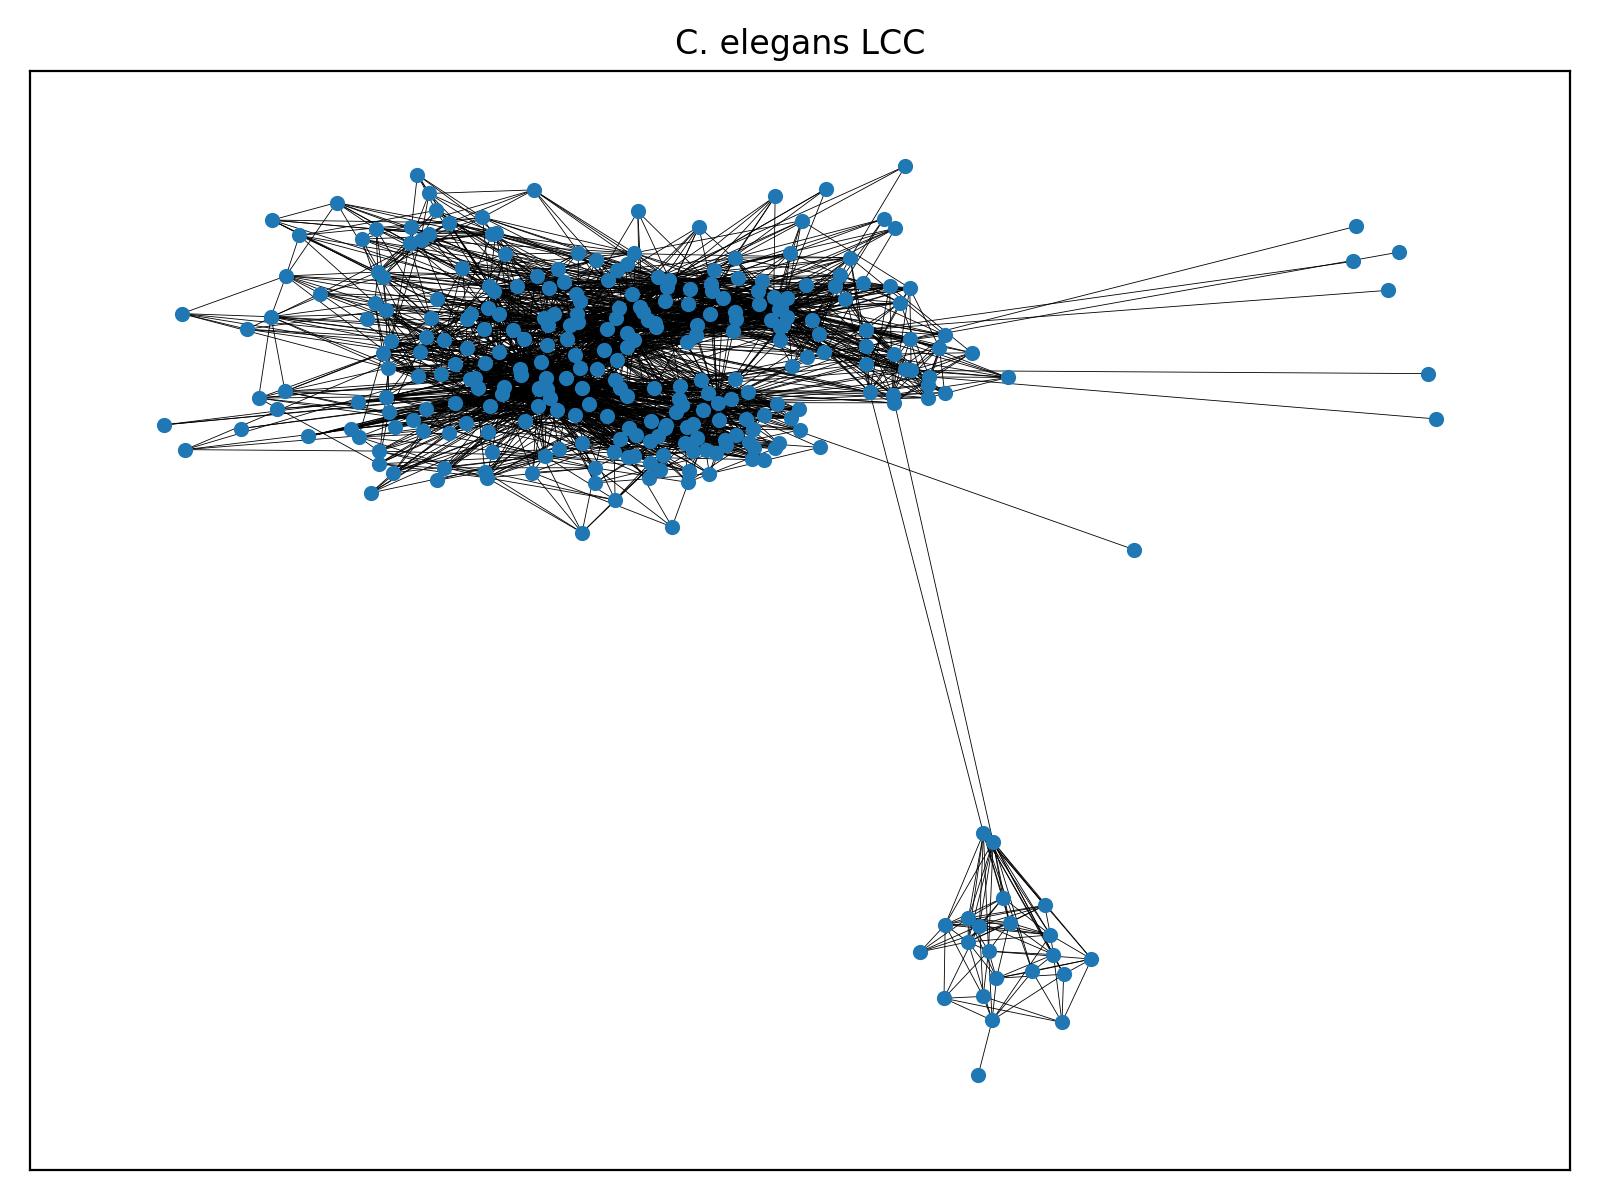
\includegraphics[width=0.92\textwidth]{real_network_visualization.png}
\caption{Spring-layout visualization of the empirical \textit{C. elegans} undirected analysis graph. High-degree nodes appear more centrally positioned. The network's visual density reflects its 2{,}511 edges; hub nodes are visible as highly connected cores.}
\label{fig:real-network}
\end{figure}

\section{Metric Comparison Across Models}

Table~\ref{tab:metric-comparison} presents the core topological metrics for all five graphs side by side. Figure~\ref{fig:metric-barplot} and Figure~\ref{fig:model-visualizations} provide visual summaries of the same comparison.

\begin{table}[H]
\centering
\caption{Topological metrics for the empirical connectome and each synthetic model. Values are computed on unweighted graphs; path lengths and diameter are computed on the largest connected component.}
\label{tab:metric-comparison}
\small
\begin{tabular}{lrrrrrrrrr}
\toprule
Network & Edges & $\langle k \rangle$ & $\sigma^2_k$ & $\langle C \rangle$ & $\langle L \rangle$ & $E_{\text{glob}}$ & $Q$ & $r$ \\
\midrule
Real & 2511 & 16.25 & 180.04 & 0.351 & 2.665 & 0.431 & 0.369 & $-0.127$ \\
Erd\H{o}s--R\'{e}nyi & 2511 & 16.25 & 14.51 & 0.052 & 2.350 & 0.459 & 0.200 & $-0.030$ \\
Regular lattice & 2472 & 16.00 & 0.00 & 0.700 & 10.130 & 0.185 & 0.550 & $ 0.000$ \\
Watts--Strogatz & 2472 & 16.00 & 4.10 & 0.261 & 2.525 & 0.430 & 0.457 & $-0.015$ \\
Barab\'{a}si--Albert & 2408 & 15.59 & 140.77 & 0.125 & 2.330 & 0.462 & 0.207 & $-0.056$ \\
\bottomrule
\end{tabular}
\end{table}

The results reveal a clear pattern: each synthetic model captures some features of the empirical connectome while missing others, often dramatically. We now examine each model in turn.

\paragraph{Erd\H{o}s--R\'{e}nyi.} The random graph matches the empirical graph exactly in node count, edge count, density, and average degree — this is by construction, since we used $G(n, m)$ with matching parameters. However, it fails on every structural metric. Its clustering coefficient (0.052) is nearly seven times lower than the biological value (0.351): in a random graph there is no tendency for neighbors to cluster together, while the biological connectome has clear local circuit organization. Its degree variance (14.5) is twelve times lower than the empirical value (180.0): random graphs have near-Poisson degree distributions, while the real graph has extreme hubs. Its assortativity ($-0.030$) is far less negative than the empirical $-0.127$. The random graph is a useful baseline precisely because it strips away all non-random structure; the large discrepancies confirm that the \textit{C. elegans} connectome is highly non-random.

\paragraph{Regular lattice.} The lattice model is the opposite failure mode. Its clustering coefficient (0.700) is twice the empirical value — it is \textit{too} clustered. More dramatically, its average path length (10.13) is nearly four times the empirical value (2.665). Neurons in a lattice must traverse many local steps to reach distant parts of the network, because there are no shortcuts. The lattice's degree variance is exactly zero: every node has exactly 16 connections, which stands in complete contrast to the biological degree heterogeneity. The lattice is also the most modular of all models ($Q = 0.550$), because adjacent nodes on the ring form natural communities. The regular lattice is the worst-ranking model overall, and its failure on path length and degree heterogeneity is particularly telling.

\paragraph{Watts--Strogatz ($p = 0.3$).} The WS model at the optimal rewiring probability represents a genuine partial success. Its path length (2.525) is close to the empirical value (2.665) — the rewired shortcuts bring distant parts of the ring within a few steps of each other. Its global efficiency (0.430) essentially matches the biological value (0.431). Its clustering (0.261), while lower than the empirical 0.351, is far higher than the random graph and the BA model, reflecting the preservation of local lattice structure. The WS model correctly identifies that the biological network is neither purely local nor purely random, and that it achieves efficient global communication without sacrificing all local organization.

Where the WS model fails is on degree heterogeneity. With degree variance of only 4.1, the WS graph has no meaningful hubs — degrees are clustered tightly around 16. It also fails on assortativity ($-0.015$ versus $-0.127$) and, to a lesser degree, on modularity (0.457 versus 0.369 — the WS graph is actually \textit{more} modular, as its community structure reflects the remnants of the ring topology).

\paragraph{Barab\'{a}si--Albert.} The BA model's most important success is in capturing degree heterogeneity. Its degree variance is 140.77 — the closest of any synthetic model to the empirical 180.04. The emergence of hubs through preferential attachment means that the model topology includes a small number of highly connected nodes, qualitatively similar to the command interneurons in the biological network. Its path length (2.330) is also short, in line with the biological graph, and its global efficiency (0.462) is similar to the empirical value. These successes are why the BA model ranks first overall.

However, the BA model is a poor match for clustering: its average clustering coefficient is only 0.125, less than one-third of the empirical 0.351. New nodes in the BA model attach to many existing nodes, but those existing nodes do not attach to each other — there is no mechanism that generates triangles. The BA model is also a poor match for modularity (0.207 versus 0.369): the hub-and-spoke structure of a BA graph does not produce strong community boundaries. And its assortativity ($-0.056$) is less negative than the empirical value, suggesting a weaker hierarchical structure than the biological connectome exhibits.

\begin{figure}[H]
\centering
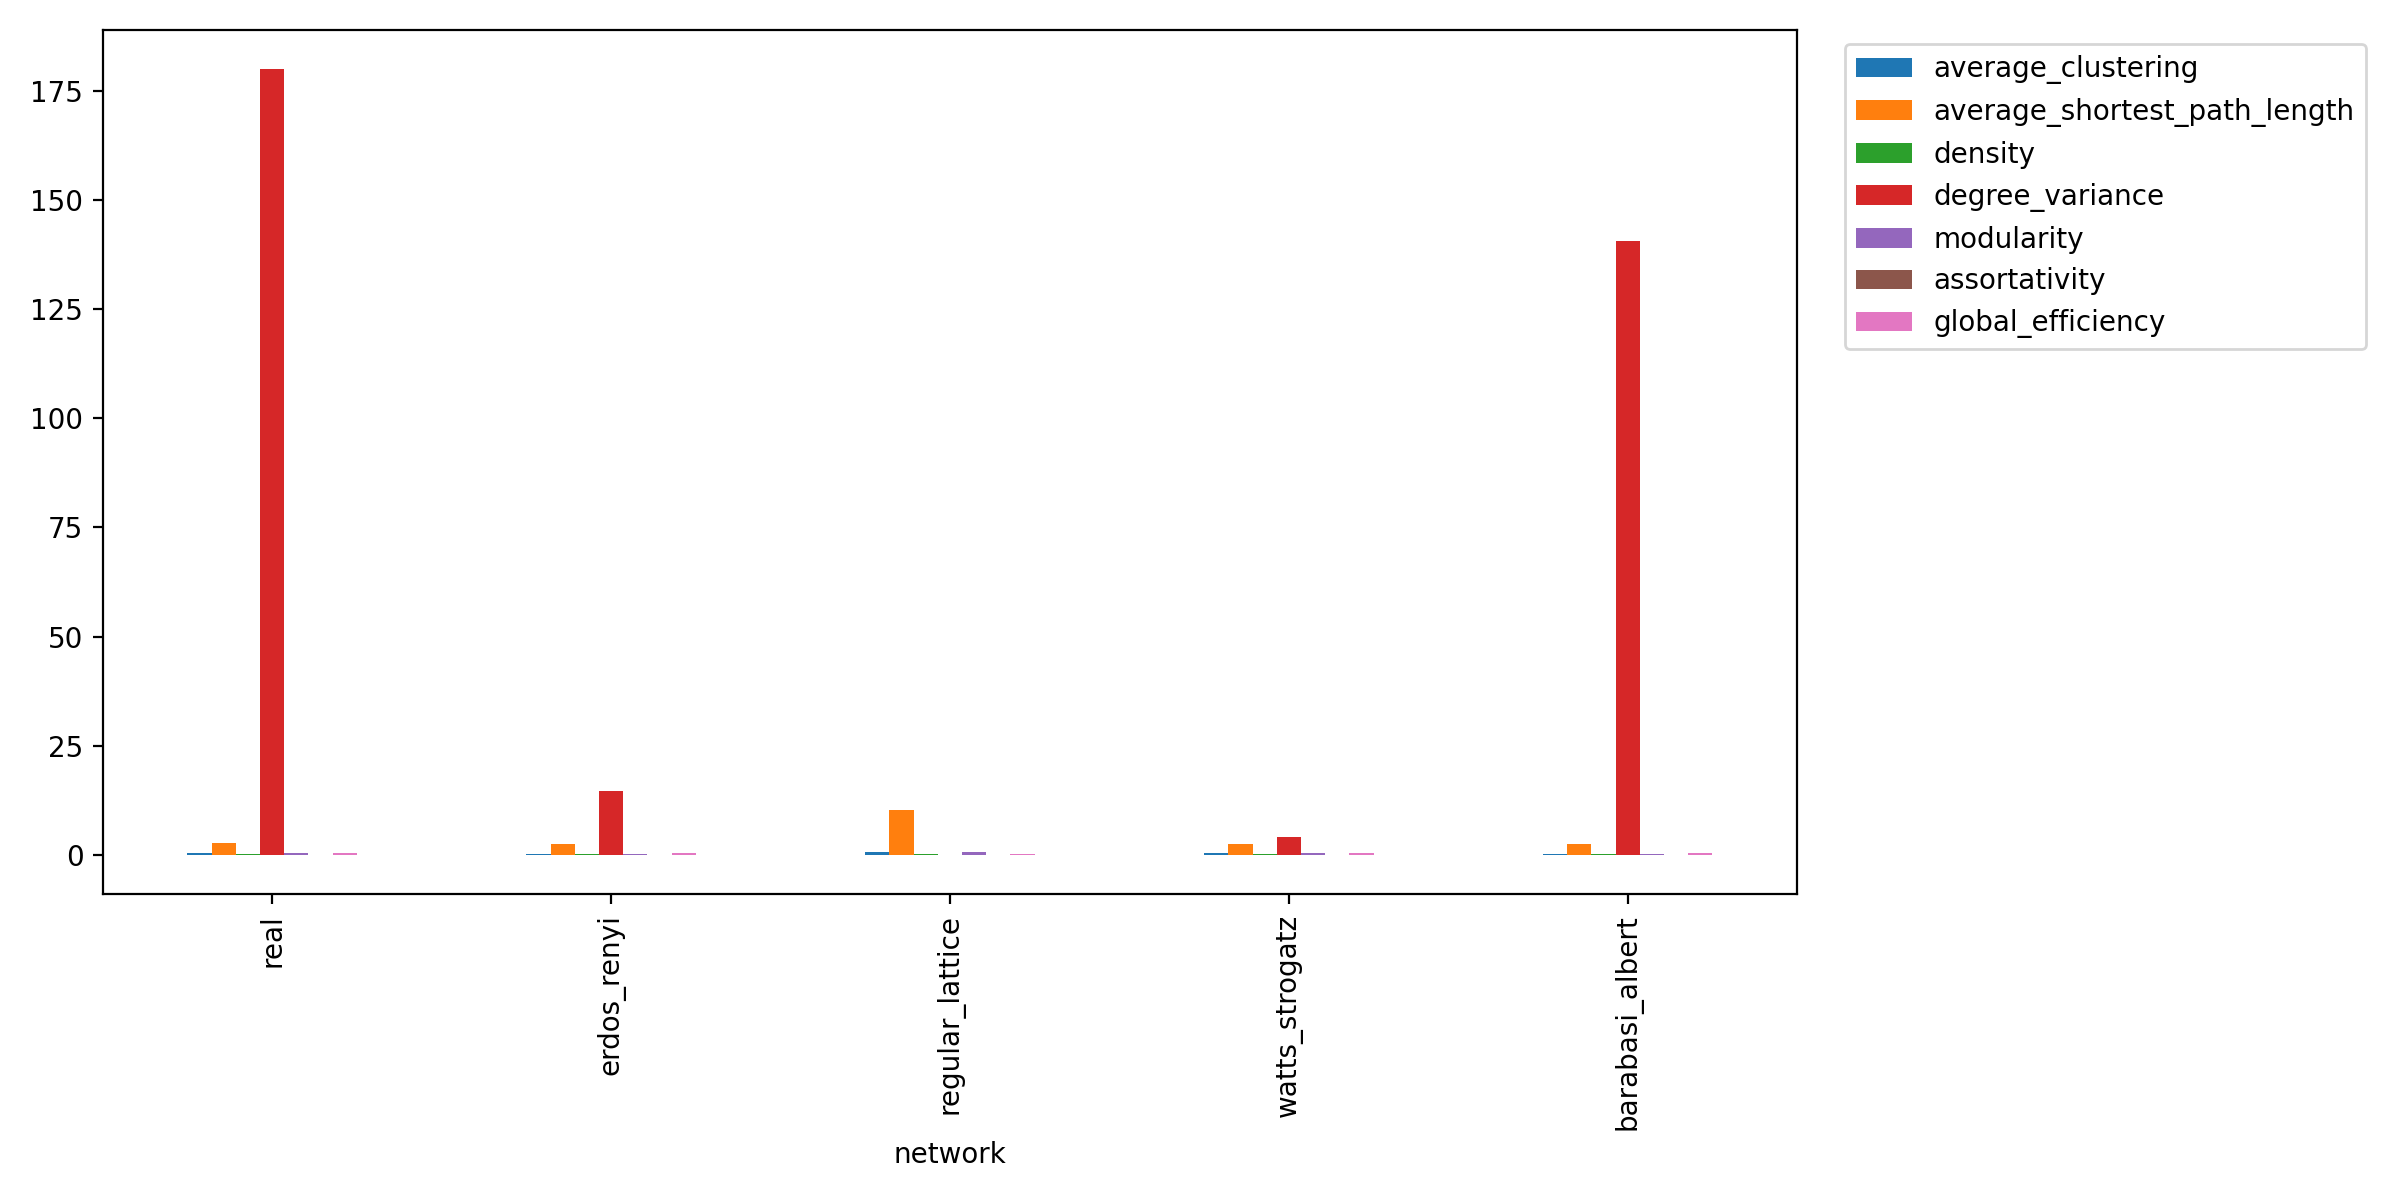
\includegraphics[width=0.98\textwidth]{metric_comparison_barplot.png}
\caption{Bar chart comparing key topological metrics across the empirical \textit{C. elegans} graph and the four synthetic models. Note that no synthetic model uniformly approximates the biological graph across all metrics.}
\label{fig:metric-barplot}
\end{figure}

\begin{figure}[H]
\centering
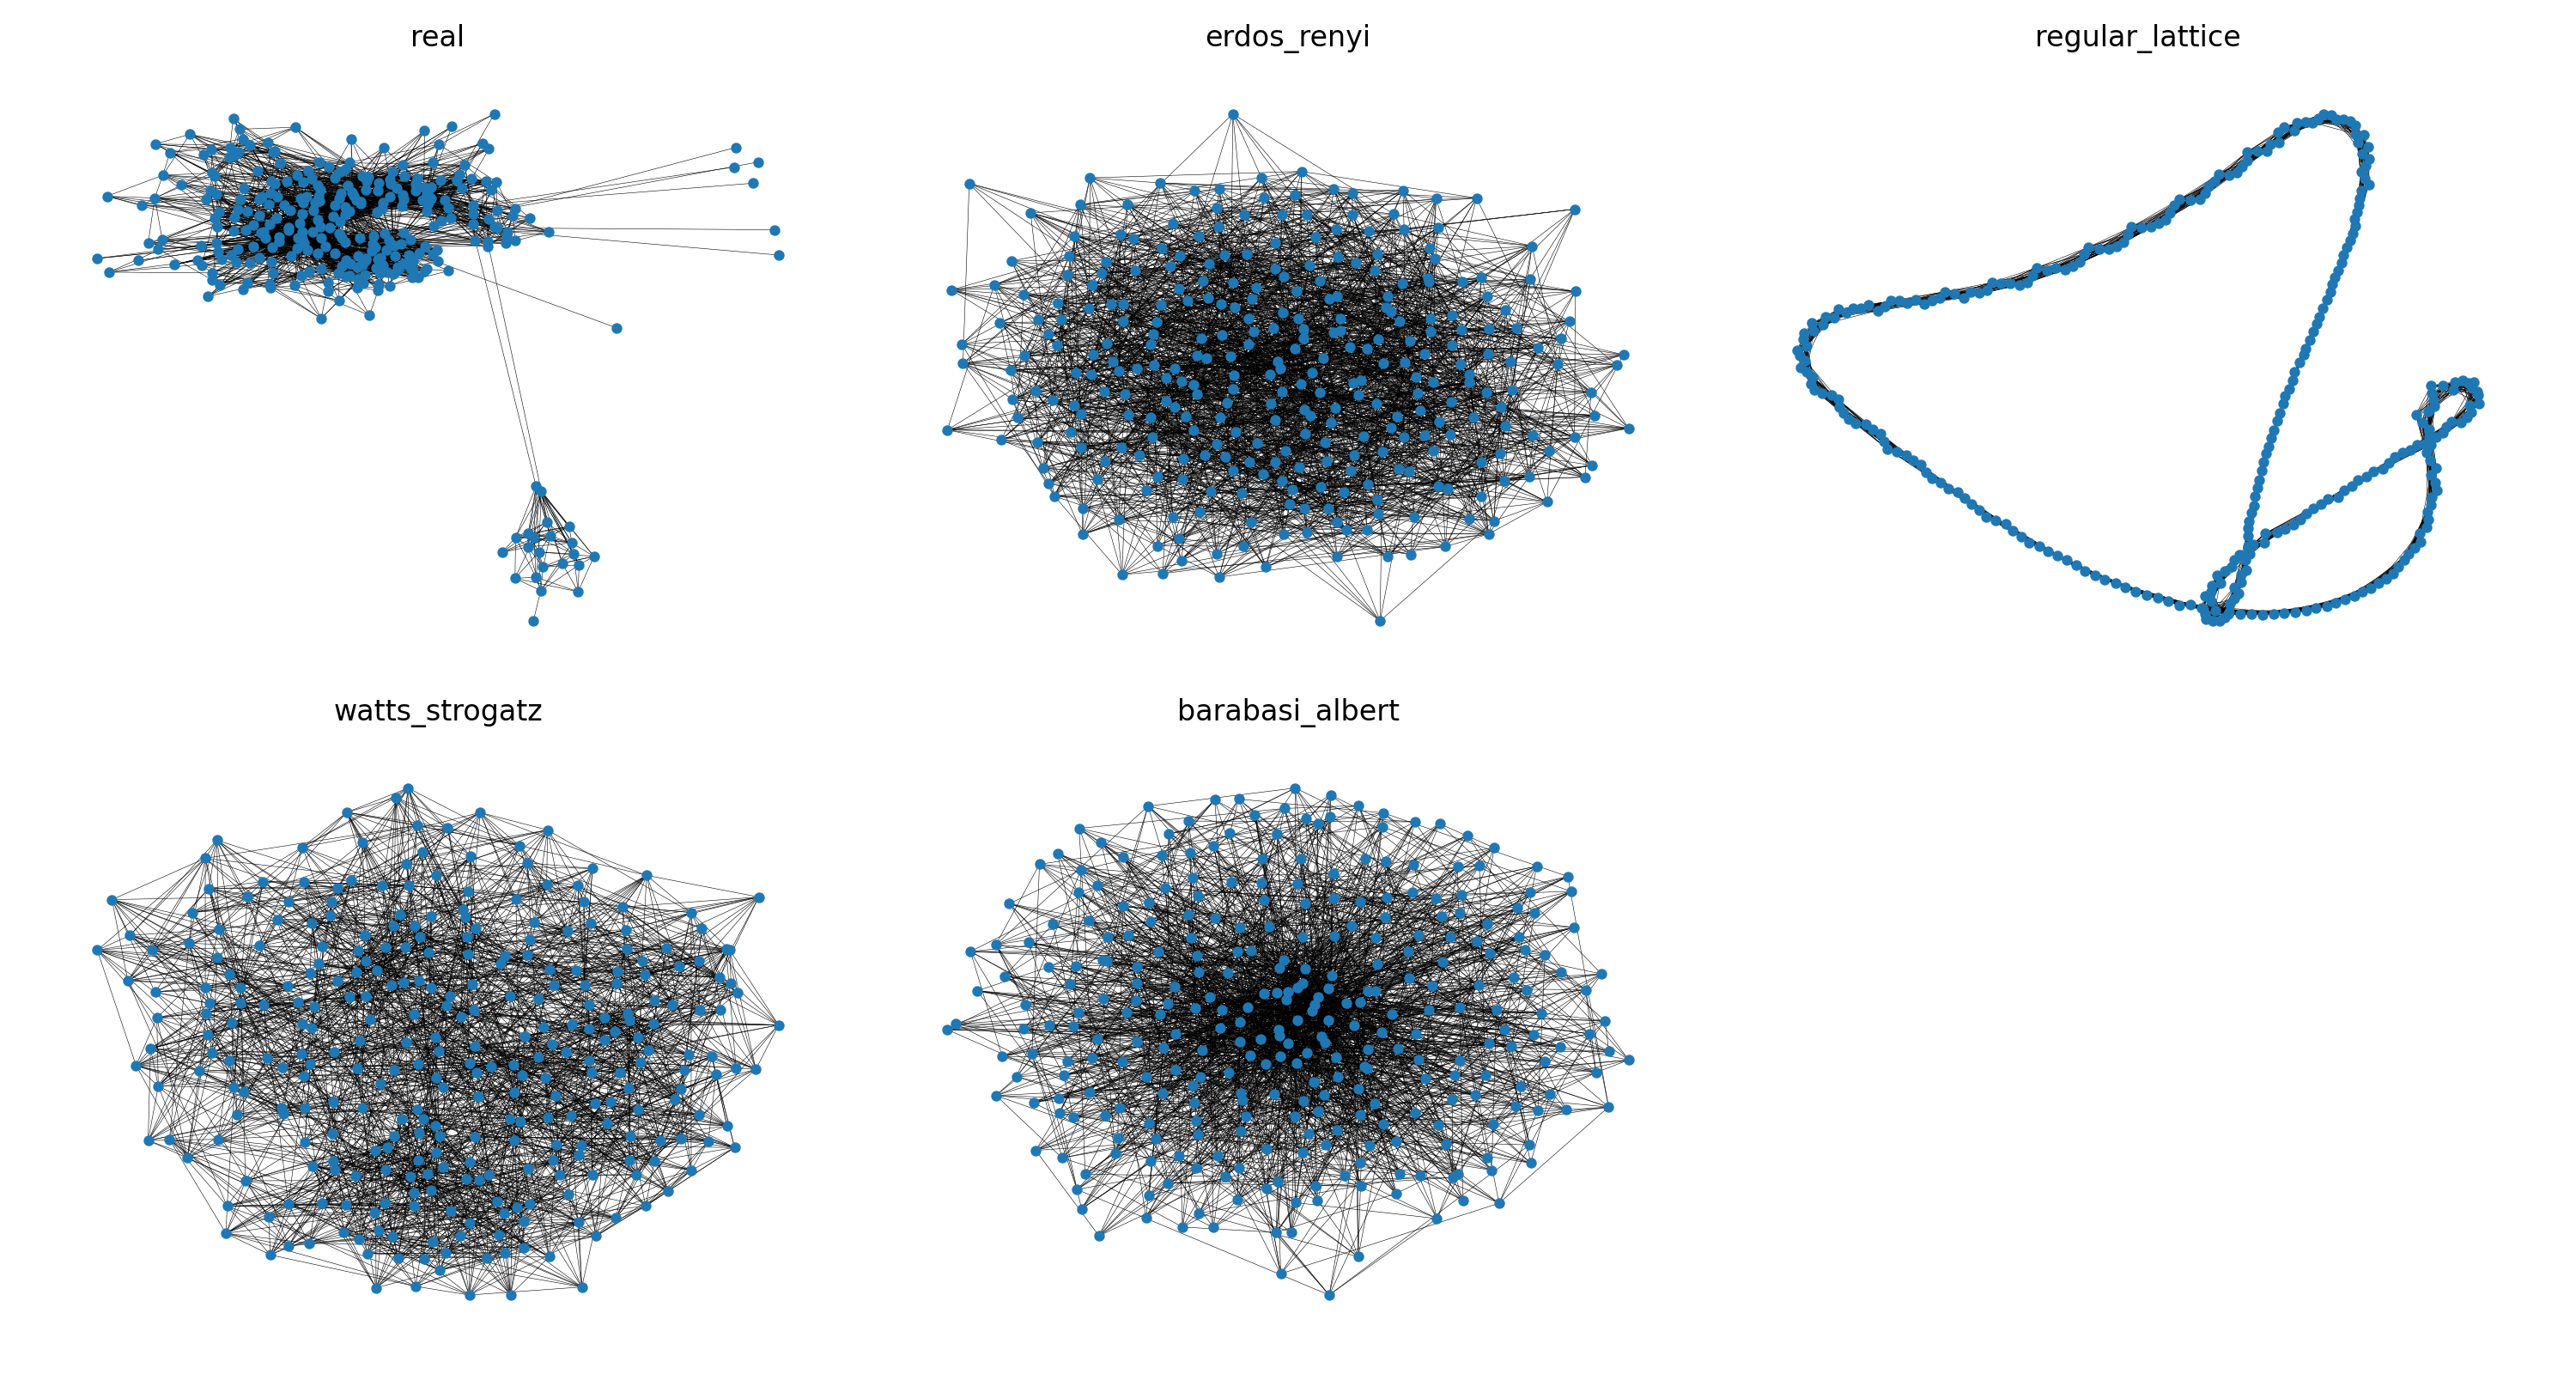
\includegraphics[width=0.98\textwidth]{model_network_visualizations.png}
\caption{Spring-layout visualizations of the empirical graph and all four synthetic models at the same scale. Visual differences in hub structure, density, and local clustering are apparent.}
\label{fig:model-visualizations}
\end{figure}

\section{Degree Distribution and Hub Structure}

\begin{figure}[H]
\centering
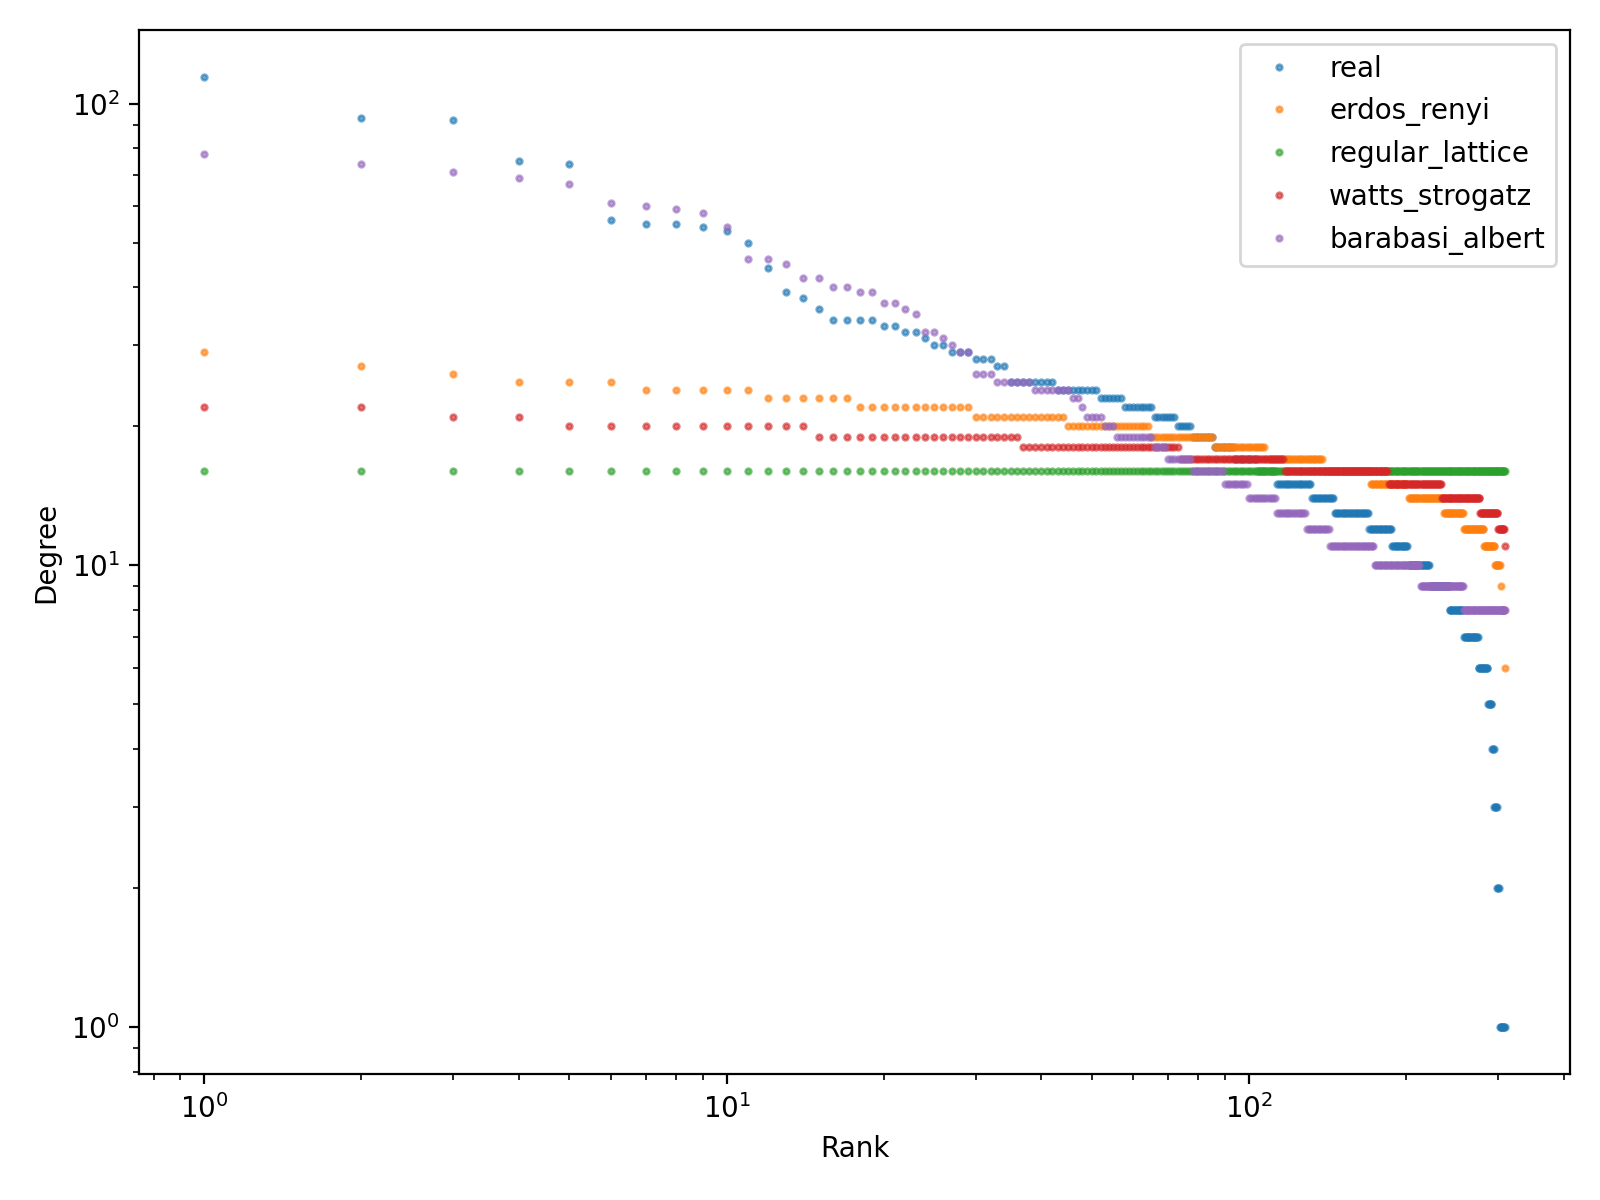
\includegraphics[width=0.92\textwidth]{degree_distribution_comparison.png}
\caption{Degree distribution histograms for the empirical graph and each synthetic model. The empirical graph and the BA model share a broad, heavy-tailed distribution. The ER and WS graphs exhibit narrow, near-Poisson distributions. The lattice is a single spike at degree 16.}
\label{fig:degree-distribution}
\end{figure}

The degree distribution plots (Figure~\ref{fig:degree-distribution}) make the hub structure comparison particularly clear. The empirical distribution has a pronounced tail, with several nodes at degree 50--114. The BA graph is the only synthetic model with a similarly long tail, though the tail shape differs in detail: the empirical distribution is not a clean power law, and the maximum degree in the BA graph (78) is lower than the empirical maximum (114, dominated by the aggregated muscle node). The ER graph has a narrow, roughly symmetric distribution centered on 16. The WS graph is nearly as narrow. The lattice distribution is a delta function at 16.

Figure~\ref{fig:centrality-distribution} shows degree centrality versus betweenness centrality for all graphs. In the empirical graph, a small subset of nodes has both high degree and high betweenness — the command interneurons. These are the network's true structural bottlenecks: they are not only well-connected but also lie on many shortest paths between other nodes. The BA graph shows a similar pattern in its highest-degree nodes, though less pronounced. The ER and WS graphs show no such concentration of betweenness at high-degree nodes.

\begin{figure}[H]
\centering
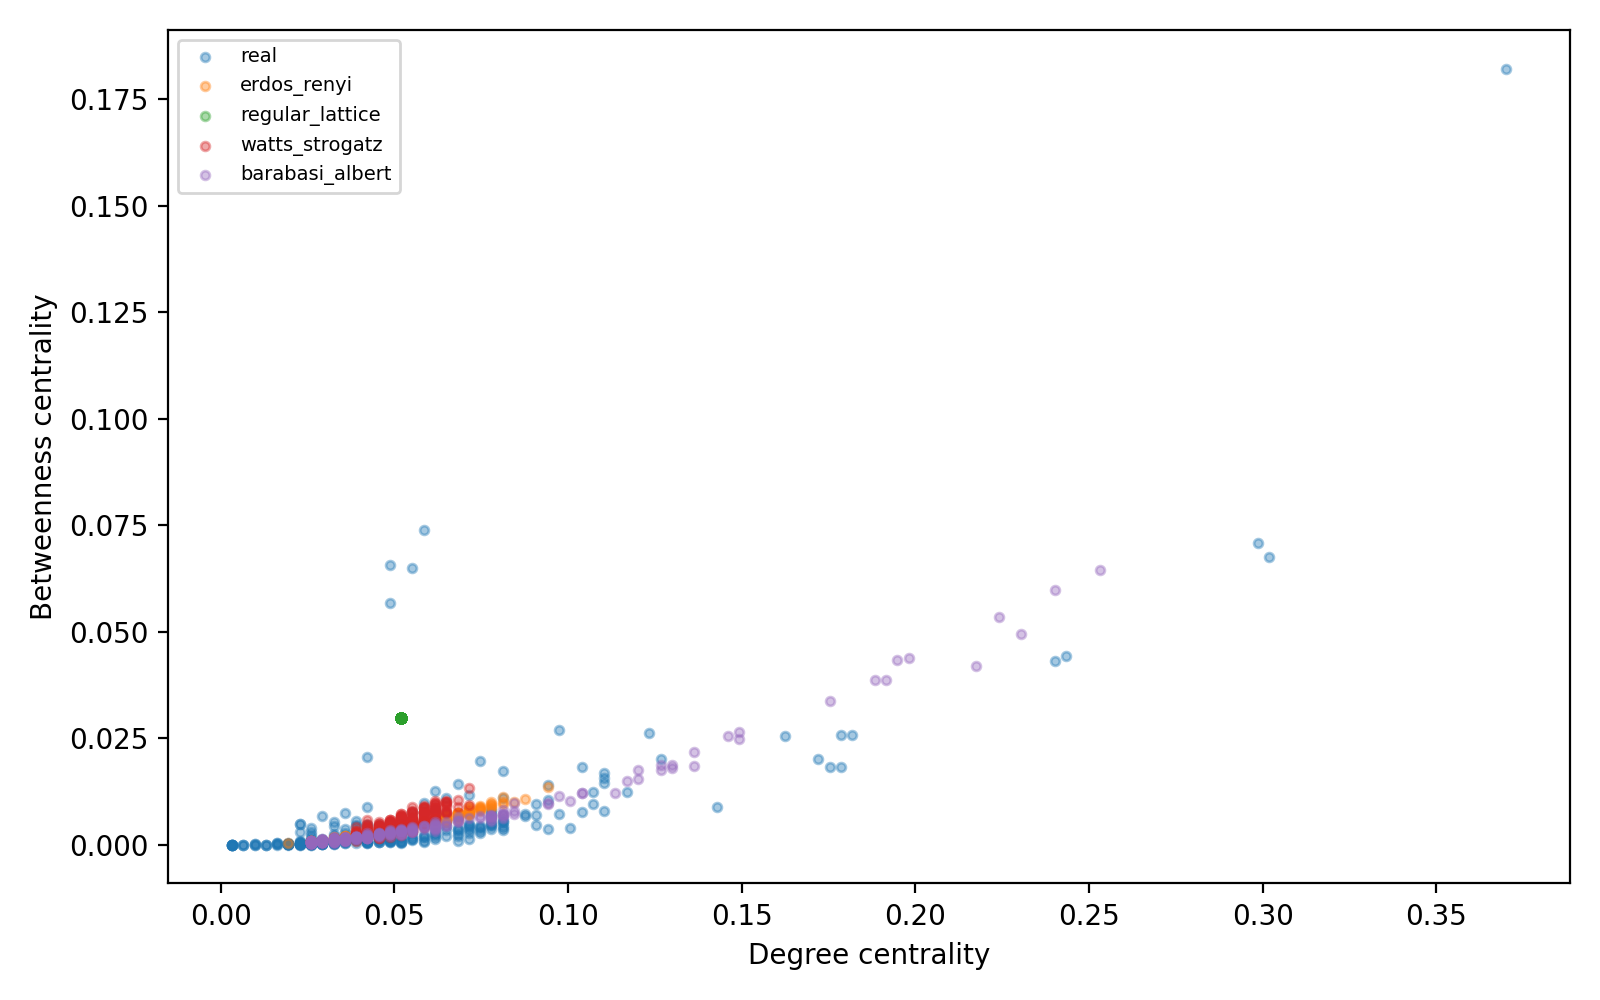
\includegraphics[width=0.92\textwidth]{centrality_distribution_comparison.png}
\caption{Scatter plots of degree centrality versus betweenness centrality for each graph. The empirical graph and, to a lesser extent, the BA graph show a small population of nodes with both high degree and high betweenness — structural hubs.}
\label{fig:centrality-distribution}
\end{figure}

\section{The Watts--Strogatz Rewiring Sweep}
\label{sec:ws-results}

Table~\ref{tab:ws-sweep} and Figure~\ref{fig:ws-sweep} document the rewiring sweep across ten values of $p$. The results trace the classic small-world transition described by Watts and Strogatz: at $p = 0$ (pure lattice), clustering is 0.700 and path length is 10.13. As $p$ increases, path length drops precipitously — already at $p = 0.005$ it has fallen to 5.65, and at $p = 0.05$ it is 3.24. Clustering decreases more slowly and smoothly. The regime $0.05 \lesssim p \lesssim 0.3$ is the small-world zone: path lengths are short but clustering remains substantially above the random-graph baseline.

The match score is minimized at $p = 0.3$, where the graph achieves a path length of 2.525 (close to the empirical 2.665) at the cost of a clustering of 0.261 (below the empirical 0.351). At $p = 0.1$, clustering is higher (0.519) but path length is longer (2.840), giving a worse combined score. This trade-off illustrates why the small-world model is the ``second-best'' synthetic approximation: it can match either the clustering or the path length of the empirical graph, but at the optimal $p = 0.3$ it undershoots clustering while approaching path length well.

It is noteworthy that the real \textit{C. elegans} clustering value (0.351) lies between the WS values at $p = 0.1$ (0.519) and $p = 0.3$ (0.261) — roughly corresponding to a rewiring probability in the range 0.1--0.3. The original Watts--Strogatz paper found $p \approx 0.05$ to be a good match for the \textit{C. elegans} connectome using a smaller dataset. Our slightly higher optimal $p$ likely reflects the larger and more complete dataset used here.

\begin{table}[H]
\centering
\caption{Watts--Strogatz rewiring sweep results. Lower match score indicates closer simultaneous agreement with the empirical clustering and path length. The optimal rewiring probability is $p = 0.3$.}
\label{tab:ws-sweep}
\small
\begin{tabular}{rrrr}
\toprule
$p$ & $\langle C \rangle$ & $\langle L \rangle$ & Match score \\
\midrule
0.000 & 0.700 & 10.130 & 7.814 \\
0.001 & 0.699 & 9.425 & 7.108 \\
0.005 & 0.693 & 5.647 & 3.324 \\
0.010 & 0.686 & 4.810 & 2.480 \\
0.030 & 0.661 & 3.790 & 1.435 \\
0.050 & 0.615 & 3.242 & 0.841 \\
0.100 & 0.519 & 2.840 & 0.343 \\
\textbf{0.300} & \textbf{0.261} & \textbf{2.525} & \textbf{0.230} \\
0.500 & 0.123 & 2.418 & 0.475 \\
1.000 & 0.048 & 2.360 & 0.607 \\
\bottomrule
\end{tabular}
\end{table}

\begin{figure}[H]
\centering
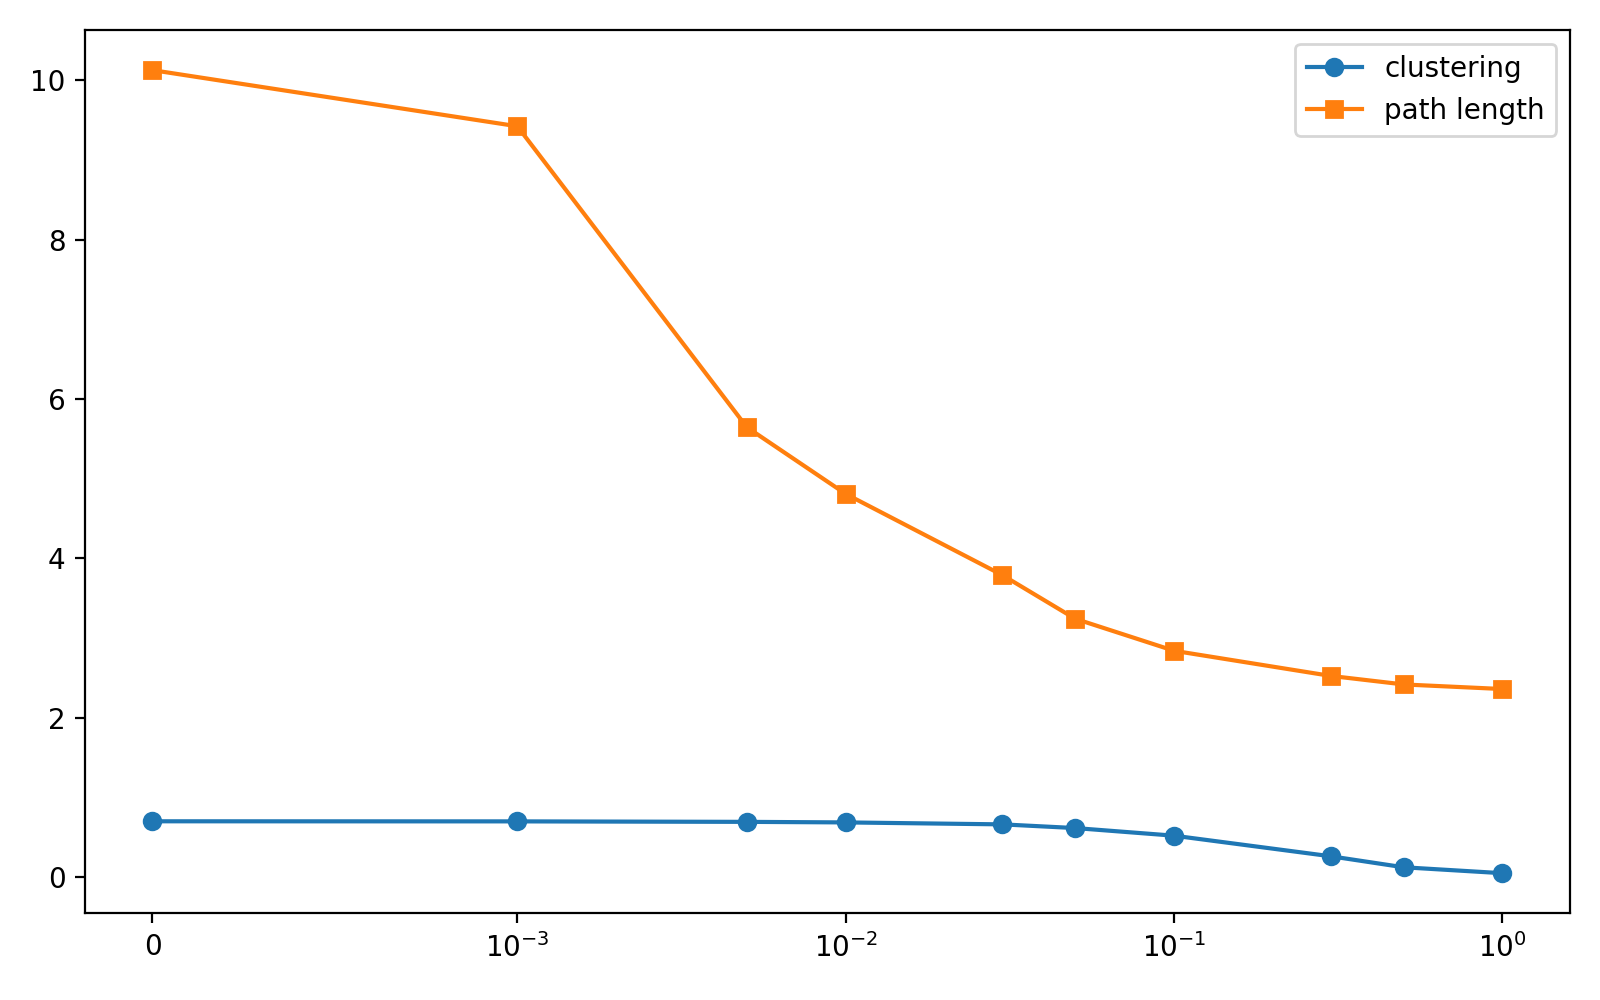
\includegraphics[width=0.92\textwidth]{clustering_vs_pathlength_ws_sweep.png}
\caption{Watts--Strogatz rewiring probability $p$ (log scale) versus average clustering (circles) and average shortest path length (squares). The small-world transition is visible: path length drops rapidly at small $p$ while clustering declines gradually. The empirical clustering (0.351) and path length (2.665) are both marked by the dashed horizontal lines (not shown on this plot, but visible in the match score table).}
\label{fig:ws-sweep}
\end{figure}

\section{Robustness Under Node Removal}

The robustness results reveal a structural asymmetry in the \textit{C. elegans} connectome that is consistent with the presence of hubs. Figure~\ref{fig:random-robustness} shows the random removal results: when nodes are removed uniformly at random, the empirical graph retains connectivity well. At 50\% random removal, 47.3\% of the original nodes remain in the largest connected component — close to the theoretical lower bound of the removal fraction itself, suggesting the graph degrades gracefully. The Erd\H{o}s--R\'{e}nyi and regular lattice graphs perform slightly better under random removal (approximately 50\% LCC fraction at 50\% removal, with near-zero variance), as expected: these graphs have no hubs to protect, so removing random nodes has the same proportional effect regardless of which nodes are chosen.

\begin{figure}[H]
\centering
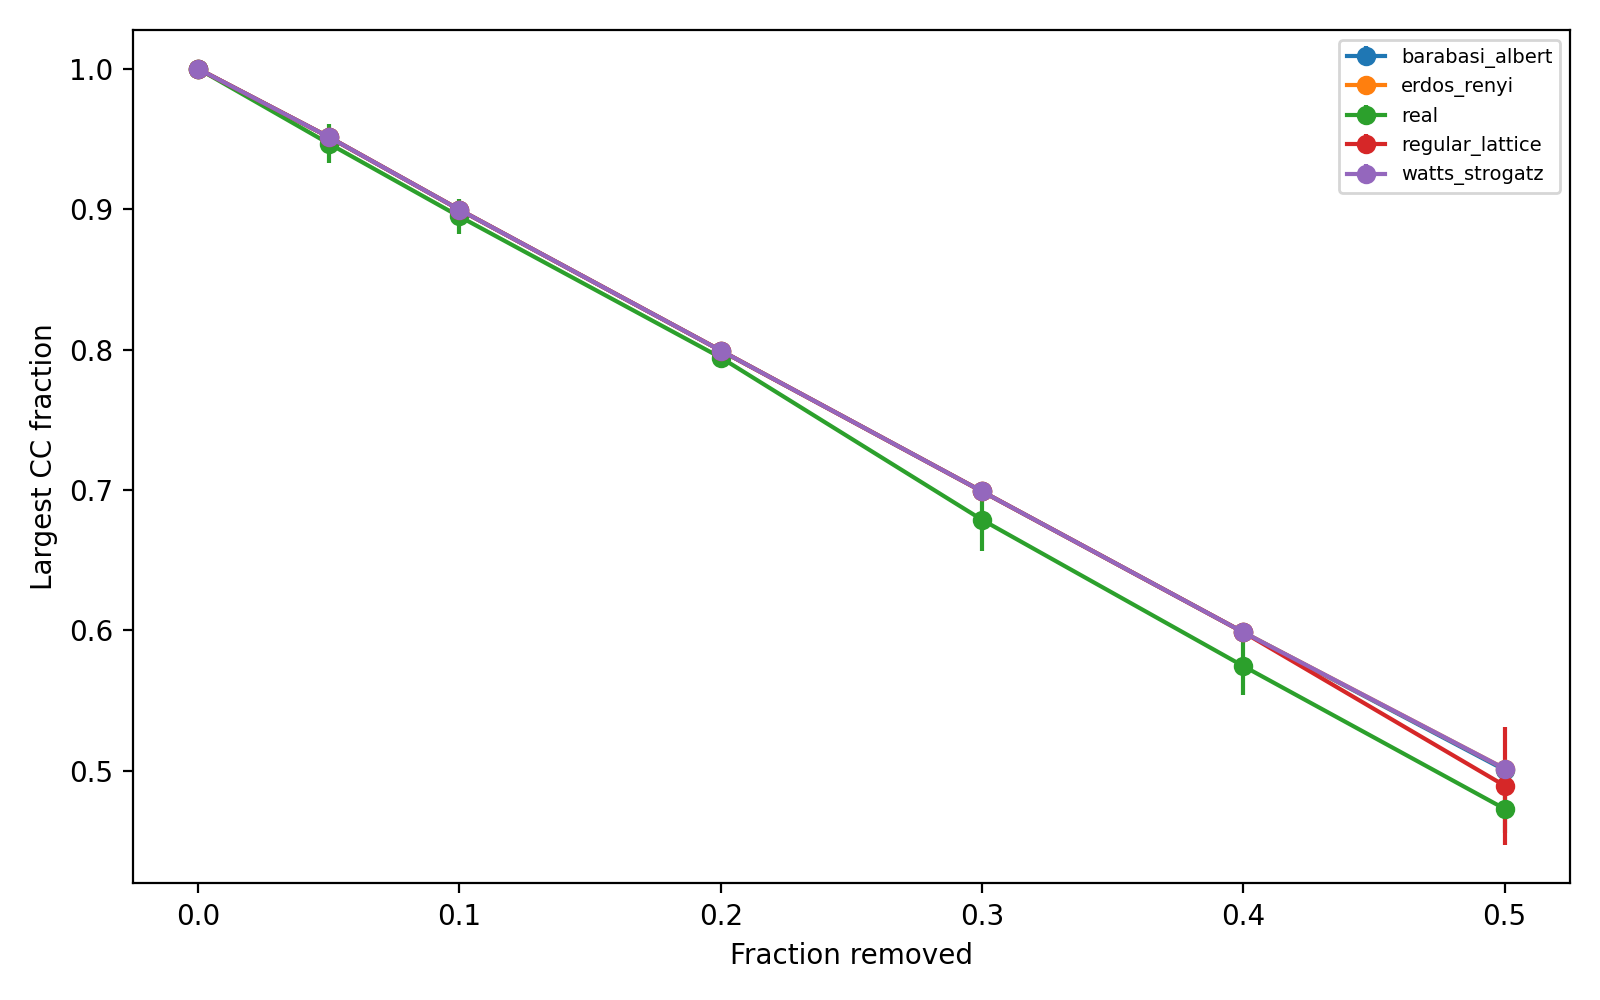
\includegraphics[width=0.92\textwidth]{robustness_random_removal.png}
\caption{Random node-removal robustness. Each curve shows the mean largest connected component fraction (as a fraction of the original $N = 309$ nodes) over 20 independent removals, with error bars indicating standard deviation. The empirical graph degrades smoothly under random removal.}
\label{fig:random-robustness}
\end{figure}

Figure~\ref{fig:targeted-robustness} tells a different story. Under targeted removal — where nodes are removed in descending order of degree — the empirical graph is far more vulnerable. Removing only the top-degree nodes rapidly fragments the network. This vulnerability to targeted attack is the defining robustness signature of hub-based networks: removing the command interneurons (AVAL, AVAR, AVBL, AVBR, etc.) severs the connections that bridge the network's communities, causing rapid disintegration. The BA model shows a qualitatively similar vulnerability, consistent with its scale-free hub structure. The regular lattice and Erd\H{o}s--R\'{e}nyi graphs are much less affected by targeted removal precisely because they have no special high-degree nodes to target.

This differential robustness pattern — resilience to random failure, vulnerability to targeted hub attack — is a hallmark of scale-free-like organization and provides independent, non-metric evidence that the hub structure in the \textit{C. elegans} connectome is functionally analogous to the hub structure in BA-generated networks.

\begin{figure}[H]
\centering
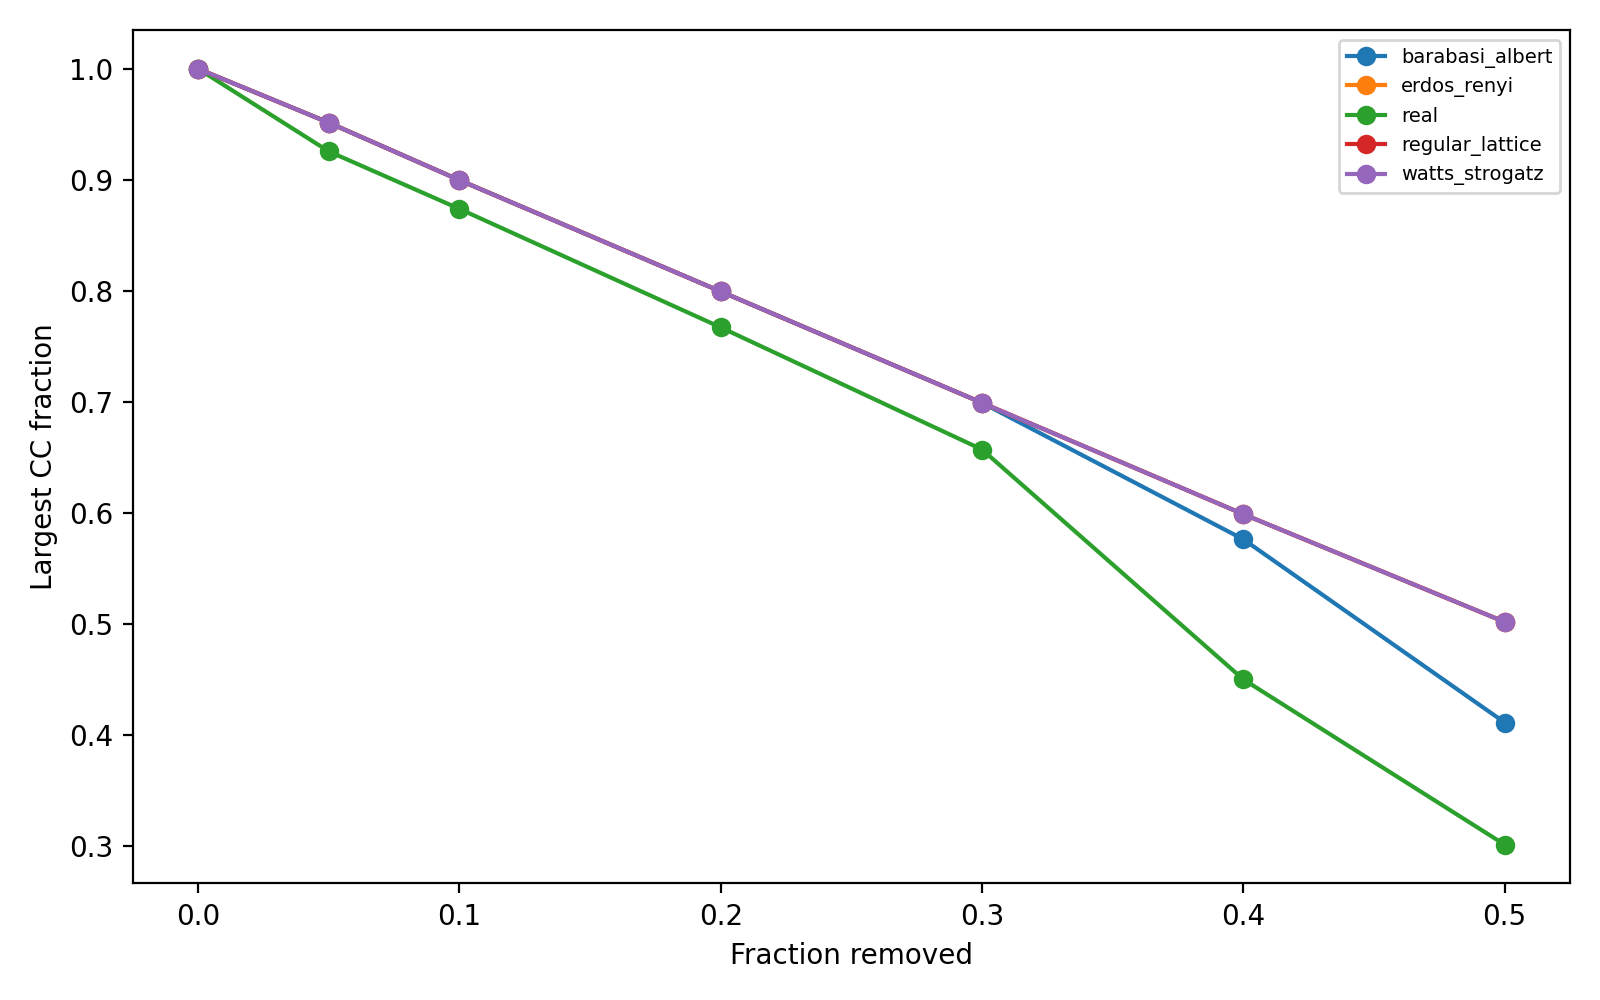
\includegraphics[width=0.92\textwidth]{robustness_targeted_removal.png}
\caption{Targeted node-removal robustness under descending-degree removal. The empirical graph and the BA model both show steep decline when hub nodes are removed first, consistent with the hub-dependent connectivity of both networks.}
\label{fig:targeted-robustness}
\end{figure}

\section{Final Model Ranking}

Table~\ref{tab:model-ranking} and Figure~\ref{fig:model-distance} present the normalized model distance ranking.

\begin{table}[H]
\centering
\caption{Normalized model-distance ranking (lower is better). The distance is the mean relative deviation across the seven selected metrics: average clustering, average path length, density, degree variance, modularity, assortativity, and global efficiency.}
\label{tab:model-ranking}
\begin{tabular}{lrrl}
\toprule
Model & Distance & Rank & Primary strength \\
\midrule
Barab\'{a}si--Albert & 0.300 & 1 & Degree heterogeneity, path length \\
Watts--Strogatz & 0.346 & 2 & Path length, global efficiency \\
Erd\H{o}s--R\'{e}nyi & 0.454 & 3 & Density (by construction) \\
Regular lattice & 0.982 & 4 & Clustering (too high) \\
\bottomrule
\end{tabular}
\end{table}

\begin{figure}[H]
\centering
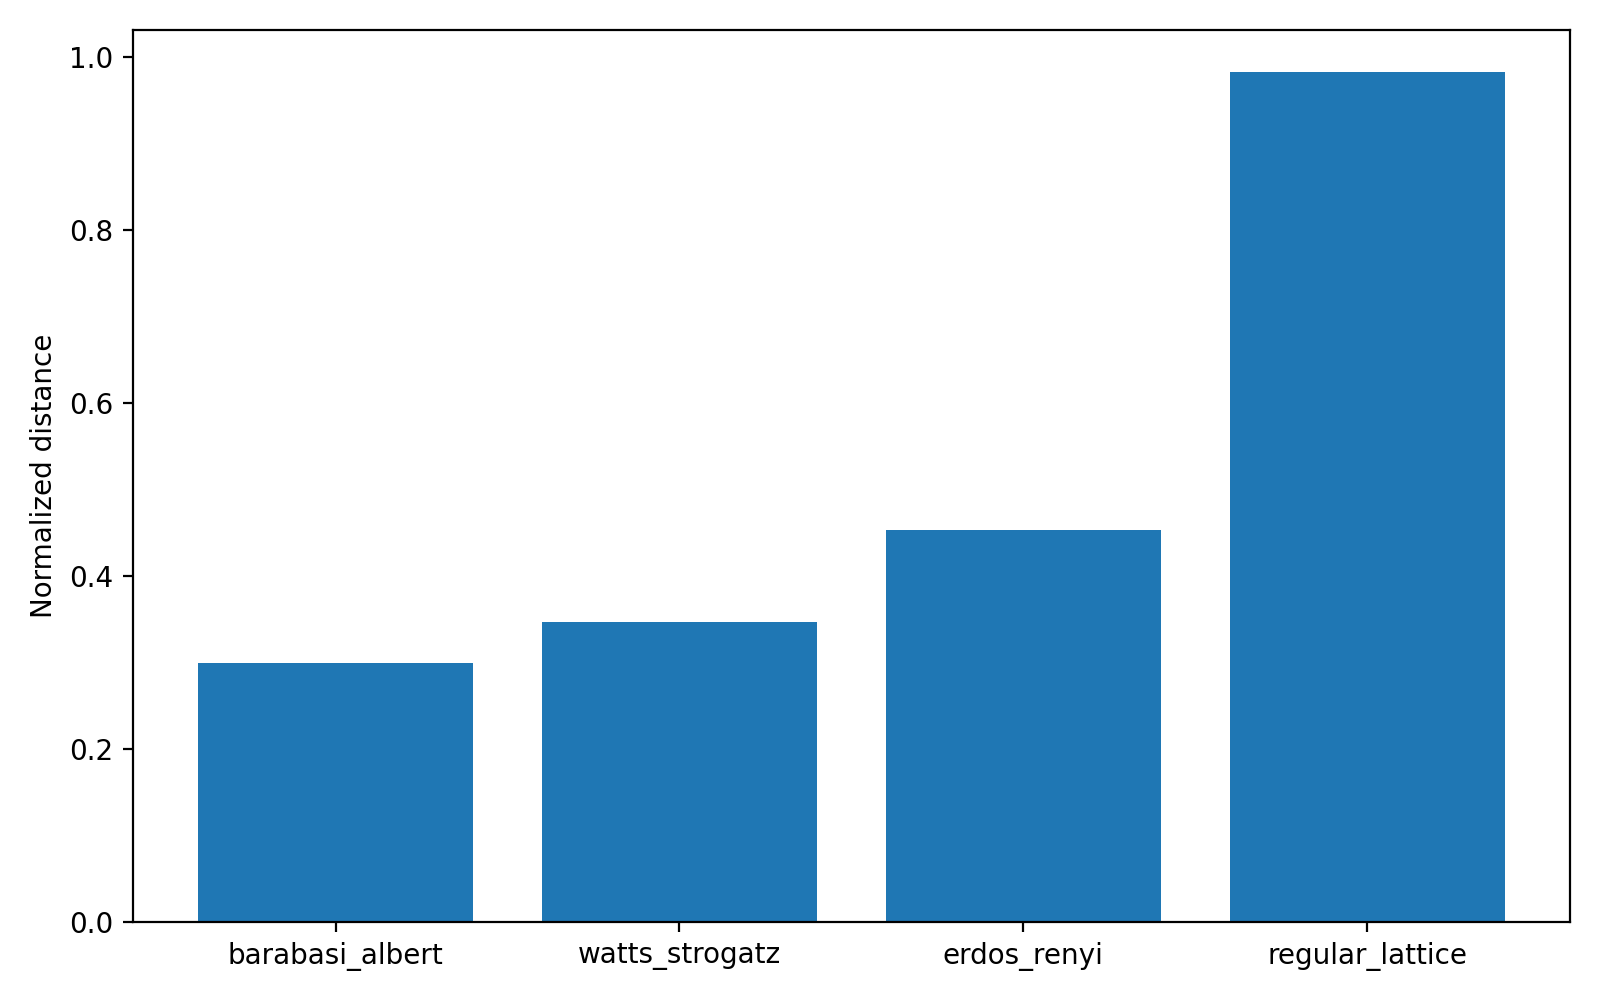
\includegraphics[width=0.82\textwidth]{model_distance_ranking.png}
\caption{Normalized metric distance scores. Lower scores indicate closer similarity to the empirical connectome. The Barab\'{a}si--Albert model ranks first, followed closely by Watts--Strogatz. The regular lattice is a distant last.}
\label{fig:model-distance}
\end{figure}

The BA model's margin over the WS model (0.300 vs 0.346) is meaningful but not overwhelming. The key difference is degree variance: the BA model's $\sigma^2_k = 140.77$ is far closer to the empirical 180.04 than the WS model's 4.10. This single metric, weighted equally with the others in the distance formula, drives the BA model's top ranking. If degree heterogeneity were weighted more heavily — as might be appropriate given how strongly it shapes both robustness and centrality structure — the gap would widen further.


%% ============================================================
\chapter{Discussion}
%% ============================================================

\section{The Scale-Free Interpretation: Strengths and Gaps}

The Barab\'{a}si--Albert model ranks first in our comparison, and the reasons for this outcome are biologically informative. The most important is degree heterogeneity. The \textit{C. elegans} connectome contains genuine functional hubs — neurons like AVAL and AVAR that connect to dozens or hundreds of other neurons — and a long-tailed degree distribution that the Poisson-like ER and WS degree distributions simply cannot reproduce. The preferential attachment mechanism of the BA model generates exactly this kind of heterogeneity, and it does so in a way that also produces short path lengths, because hubs serve as efficient routing nodes.

The robustness experiments reinforce this interpretation. The empirical graph's differential robustness — graceful degradation under random removal but rapid fragmentation under hub-targeted removal — is the characteristic fingerprint of hub-based organization, and it is reproduced qualitatively by the BA model. This is an important consistency check: the BA model's match to the empirical graph is not an artifact of the particular metric set chosen, but reflects a deep structural property.

However, the scale-free interpretation has important limitations. The BA model's clustering coefficient (0.125) is less than one-third of the empirical value (0.351). The mechanism of preferential attachment does not create triangles: a new node connects to many already-connected hubs, but those hubs do not thereby connect to each other. The result is a hub-and-spoke architecture with low local cohesion. The biological connectome, in contrast, has substantial local circuit organization: neurons that share a hub also tend to connect to each other, forming dense local processing clusters that are invisible in a pure BA graph.

The BA model also misses the modularity of the biological graph. The empirical $Q = 0.369$ with four clearly defined communities is substantially stronger than the BA model's $Q = 0.207$. In a BA graph, hubs attract connections from across the graph, suppressing natural community boundaries. The \textit{C. elegans} connectome, by contrast, organizes its connections into functionally coherent sub-circuits, a property that the BA mechanism does not account for.

Finally, the disassortativity of the empirical graph ($r = -0.127$) is stronger than any of the synthetic models reproduce, including the BA model ($r = -0.056$). This stronger disassortativity suggests a more pronounced hierarchical circuit structure in the biological graph than the BA mechanism generates: hubs are even more strongly biased toward connecting to peripheral neurons than would arise from preferential attachment alone.

\section{The Small-World Interpretation: A Complementary Perspective}

The Watts--Strogatz model's second-place ranking reflects a genuine insight about the \textit{C. elegans} connectome. The combination of short path lengths and substantial clustering — the small-world property — is real and was one of the first non-trivial topological findings about the \textit{C. elegans} nervous system. The WS model captures this efficiently: a relatively modest rewiring probability ($p = 0.3$) is sufficient to reduce path lengths from the lattice's 10.13 to 2.52, approaching the empirical 2.665.

What the WS model misses is exactly what the BA model captures: degree heterogeneity. A WS graph has degree variance of 4.10 regardless of the rewiring probability — the rewiring occasionally changes the degree of individual nodes, but never produces the massive hubs that the biological graph contains. The WS model therefore accurately describes the \textit{efficiency} of signal propagation across the \textit{C. elegans} nervous system but fails to describe its organizational hierarchy.

There is also an interesting mismatch in the assortativity dimension. WS graphs are nearly neutral ($r = -0.015$), while the biological graph is strongly disassortative ($r = -0.127$). This difference is structurally important: in a WS graph there is no preferred pattern of which nodes connect to which, while in the biological graph hubs systematically connect to non-hubs, creating a hierarchical architecture that the small-world model does not model.

\section{The Hybrid Interpretation: Beyond Any Single Model}

The most scientifically meaningful result of this analysis is not the ranking itself but the pattern of partial matches. No canonical model captures all of the empirical connectome's features simultaneously. The BA model captures hub structure and robustness asymmetry but misses clustering and modularity. The WS model captures path efficiency and some clustering but misses hubs and disassortativity. The ER model matches density by construction but misses everything else. The lattice model captures only the high clustering that neither random-based model achieves.

This pattern is not a failure of the analysis — it is the result. The \textit{C. elegans} connectome is a hybrid complex network. It has:

\begin{itemize}
    \item \textbf{Hub structure} (from scale-free-like organization): a small set of command interneurons that accumulate far more connections than the average, enabling integration across the whole nervous system.
    \item \textbf{Short paths and efficient communication} (from small-world organization): any two neurons are separated by at most eight synaptic steps, and typically fewer than three, enabling rapid propagation of signals from sensory inputs to motor outputs.
    \item \textbf{Local clustering and circuit identity} (from lattice-like local structure): neurons that share a functional role tend to be densely interconnected locally, forming identifiable circuits that are preserved even across individual animals.
    \item \textbf{Modular organization} (not captured by any canonical model): the connectome decomposes into four relatively distinct communities that likely reflect broad functional divisions of the nervous system.
    \item \textbf{Disassortative mixing} (partially captured by BA, but stronger in the data): hubs connect preferentially to low-degree neurons, supporting a hierarchical flow of information from peripheral sensory cells to integrating command interneurons to motor output.
\end{itemize}

This combination of features is not accidental. It reflects the functional demands of a compact nervous system that must simultaneously support local circuit computations (requiring clustering), global rapid coordination (requiring short paths and hubs), specialized subsystem identity (requiring modularity), and hierarchical signal integration (requiring disassortativity). Canonical network models, which are built to illustrate one principle at a time, cannot be expected to reproduce all of these features simultaneously.

\section{Connecting Topology to Biology}

It is worth pausing to note that the identified hubs — AVAL, AVAR, AVBL, AVBR — are not hubs by coincidence. They are the command interneurons of the locomotion circuit, and their high connectivity is a direct structural consequence of their functional role. To coordinate forward or backward movement of the entire body, a command neuron must receive input from diverse sensory modalities and project output to dozens of motor neurons distributed along the ventral cord. The high degree is not a statistical accident; it is the architectural signature of a functional integrator.

The aggregated node \texttt{LegacyBodyWallMuscles} presents a complication in this interpretation. With degree 114, it ranks above any individual neuron — but this is partly an artifact of how the data represents muscle connectivity. Body wall muscles receive input from many motor neurons and are therefore highly connected in the circuit graph, but the aggregation of many individual muscle cells into a single node artificially inflates this connectivity in the undirected projection. This does not invalidate the hub analysis for the neuronal nodes, but it is a reminder that the topology of the graph is sensitive to the choice of granularity in node definition.

%% ============================================================
\chapter{Limitations}
\label{sec:limitations}
%% ============================================================

Several important limitations qualify the conclusions of this analysis.

\paragraph{Undirected, unweighted topology.} The most significant simplification is the use of an undirected, unweighted graph projection. Synaptic connections in \textit{C. elegans} are directed: chemical synapses transmit signals only from presynaptic to postsynaptic neurons. Information flow in the nervous system follows this directionality. By projecting to an undirected graph, we discard the distinction between input and output connectivity of each neuron. Similarly, by ignoring synapse counts, we treat all edges as equal regardless of whether a connection involves one synapse or thirty. Both simplifications are necessary for a fair comparison with the undirected canonical models, but they mean that our topological metrics describe the \textit{potential connectivity structure} rather than the actual signal-transmission architecture.

\paragraph{Single biological dataset.} This analysis is based on one connectome dataset from one organism at one developmental stage. The \textit{C. elegans} connectome has been reconstructed independently by multiple groups, and there are quantitative differences between reconstructions. More importantly, even if this dataset is an accurate snapshot of the adult hermaphrodite connectome, it does not speak to variation across individuals, variation with developmental stage, or variation with environmental conditions. Whether other organisms' connectomes show the same hybrid topological features is a separate empirical question.

\paragraph{Single synthetic graph instances.} Each synthetic model was compared to the empirical graph using a single generated instance (with fixed seed 42). Stochastic graph models — especially ER and WS — can show substantial instance-to-instance variation in some metrics (particularly assortativity and community structure in smaller graphs). A more statistically rigorous comparison would generate many instances of each model, compute metric distributions, and test whether the empirical values fall within the expected ranges of each distribution. Our point-estimate comparison is informative but does not provide this distributional characterization.

\paragraph{Metric selection and weighting.} The normalized distance metric treats seven selected metrics with equal weight. Different weighting choices can change the ranking. For instance, if clustering were given double weight, the gap between BA and WS would narrow; if degree variance were given double weight, the gap would widen. The metric set itself excludes several potentially informative quantities: rich-club coefficient, motif frequencies, spectral properties, and weighted analogs of clustering and path length. The ranking should be interpreted as specific to the chosen metric set and weighting, not as a universal verdict.

\paragraph{Canonical models as simplified baselines.} The four models compared here represent foundational ideas in network science, but they are not the only models available. Biologically motivated generative models — such as spatial network models, exponential random graphs conditioned on degree sequences, or hierarchical modular networks — might provide much closer approximations to the biological connectome. The question ``which of these four canonical models is closest?'' is answerable, but it is a narrower question than ``what generative model best explains the \textit{C. elegans} connectome?''

%% ============================================================
\chapter{Conclusion}
%% ============================================================

This project asked which canonical complex network model — random, lattice, small-world, or scale-free — best approximates the topology of a real biological neural network. Using the \textit{C. elegans} connectome from the OpenWorm ConnectomeToolbox dataset and a normalized multi-metric distance score over seven topological metrics, we find that the Barab\'{a}si--Albert scale-free model is the closest approximation (distance 0.300), followed by the Watts--Strogatz small-world model (0.346), the Erd\H{o}s--R\'{e}nyi random graph (0.454), and the regular lattice (0.982).

The strongest conclusion of this analysis is not the ranking itself, but the interpretation that motivates it: the \textit{C. elegans} connectome is a genuine hybrid complex network that does not conform to any single canonical model. The Barab\'{a}si--Albert model wins the comparison because degree heterogeneity — the hub structure of the command interneurons — is the dominant topological feature that separates the biological network from all alternatives, and it is a feature that only the preferential-attachment mechanism reproduces. The Watts--Strogatz model earns second place because the biological network also has the short path lengths and substantial clustering characteristic of small-world organization. But no model captures clustering, hub structure, modularity, disassortativity, and path efficiency simultaneously, because no canonical model was designed to.

The biological lesson is that the \textit{C. elegans} nervous system is organized according to multiple concurrent principles: integration efficiency through hubs, local circuit coherence through clustering, functional segregation through modularity, and hierarchical signal flow through disassortativity. These principles are not independent — they are co-selected by evolution to produce a nervous system that can sense the environment, integrate signals rapidly, coordinate whole-body movement, and do all of this with exactly 302 neurons and a metabolically affordable number of synapses. The topology of the connectome is not a byproduct of its development but a functional architecture, and understanding it requires the vocabulary of both canonical network models and the biology they imperfectly but usefully approximate.

%% ============================================================
\chapter{Future Directions}
%% ============================================================

This analysis opens several directions for more detailed investigation:

\begin{itemize}
    \item \textbf{Directed and weighted analysis.} Repeating the comparison on the directed graph, with metrics adapted for directionality (in-degree vs. out-degree distributions, strongly connected components, directed path lengths, reciprocity), would test whether the hub structure and disassortativity persist when synaptic directionality is preserved.

    \item \textbf{Separation by connection type.} The dataset distinguishes chemical synapses from gap junctions (electrical synapses). These two types have different functional properties: gap junctions are bidirectional and fast; chemical synapses are directional and computationally richer. Comparing separate subgraphs for each connection type would reveal whether the small-world and scale-free properties are shared between the two modalities or concentrated in one.

    \item \textbf{Ensemble comparison with statistical testing.} Generating large ensembles (100+ instances) of each synthetic model and comparing metric distributions to the empirical values using appropriate statistical tests would establish which differences are statistically significant versus within the random fluctuation expected for that model class.

    \item \textbf{Rich-club and motif analysis.} Rich-club analysis would test whether the identified hubs form a densely interconnected core — a ``rich club'' — or whether they connect mainly to peripheral neurons (consistent with the disassortativity). Network motif analysis would identify local connectivity patterns (three- and four-node subgraphs) that appear more or less frequently than expected by chance, which can reveal functional circuit elements.

    \item \textbf{Biologically motivated generative models.} Beyond the four canonical models, spatially embedded network models that account for the physical layout of the nematode body, or exponential random graph models constrained to the observed degree sequence, might approximate the \textit{C. elegans} connectome much more closely. Benchmarking against such models would address the question of which biological constraints are most important for explaining the observed topology.

    \item \textbf{Cross-species comparison.} Applying the same pipeline to the \textit{Drosophila} larval connectome (which has also been fully reconstructed at the synaptic level) would test whether the hybrid topological character of the \textit{C. elegans} connectome is a universal feature of small complete nervous systems or a species-specific property.
\end{itemize}

%% ============================================================
\appendix
\chapter{Generated Pipeline Artifacts}
%% ============================================================

\section{Figures}

The following figures are produced by the analysis pipeline and incorporated into this report:

\begin{itemize}
    \item \texttt{real\_network\_visualization.png} — spring-layout visualization of the empirical connectome
    \item \texttt{model\_network\_visualizations.png} — side-by-side visualizations of all five graphs
    \item \texttt{degree\_distribution\_comparison.png} — degree distribution histograms
    \item \texttt{clustering\_vs\_pathlength\_ws\_sweep.png} — WS parameter sweep visualization
    \item \texttt{metric\_comparison\_barplot.png} — multi-metric bar chart comparison
    \item \texttt{centrality\_distribution\_comparison.png} — degree vs.\ betweenness centrality scatter plots
    \item \texttt{robustness\_random\_removal.png} — random node-removal robustness curves
    \item \texttt{robustness\_targeted\_removal.png} — targeted node-removal robustness curves
    \item \texttt{model\_distance\_ranking.png} — final model ranking bar chart
\end{itemize}

\section{Tables}

The following CSV tables are written by the pipeline to \texttt{results/tables/}:

\begin{itemize}
    \item \texttt{real\_network\_summary.csv} — dataset provenance and basic graph statistics
    \item \texttt{all\_metrics\_comparison.csv} — full metric table for all five graphs
    \item \texttt{model\_distance\_ranking.csv} — normalized distance scores and ranks
    \item \texttt{ws\_sweep\_results.csv} — WS rewiring sweep results for all tested $p$ values
    \item \texttt{robustness\_random.csv} — random removal LCC means and standard deviations
    \item \texttt{robustness\_targeted.csv} — targeted removal LCC fractions
\end{itemize}

%% ============================================================
\begin{thebibliography}{99}
%% ============================================================

\bibitem{white1986structure}
J.~G. White, E.~Southgate, J.~N. Thomson, and S.~Brenner.
\newblock The structure of the nervous system of the nematode \textit{Caenorhabditis elegans}.
\newblock \textit{Philosophical Transactions of the Royal Society of London. Series B, Biological Sciences}, 314(1165):1--340, 1986.
\newblock \url{https://doi.org/10.1098/rstb.1986.0056}.

\bibitem{openwormtoolbox}
OpenWorm Foundation.
\newblock ConnectomeToolbox data repository.
\newblock \url{https://github.com/openworm/ConnectomeToolbox}. Accessed May 2026.

\bibitem{erdos1959random}
P.~Erd\H{o}s and A.~R\'{e}nyi.
\newblock On random graphs.
\newblock \textit{Publicationes Mathematicae}, 6:290--297, 1959.

\bibitem{watts1998collective}
D.~J. Watts and S.~H. Strogatz.
\newblock Collective dynamics of `small-world' networks.
\newblock \textit{Nature}, 393:440--442, 1998.
\newblock \url{https://doi.org/10.1038/30918}.

\bibitem{barabasi1999emergence}
A.-L. Barab\'{a}si and R.~Albert.
\newblock Emergence of scaling in random networks.
\newblock \textit{Science}, 286(5439):509--512, 1999.
\newblock \url{https://doi.org/10.1126/science.286.5439.509}.

\bibitem{newman2010networks}
M.~E.~J. Newman.
\newblock \textit{Networks: An Introduction}.
\newblock Oxford University Press, Oxford, 2010.

\bibitem{latora2001efficient}
V.~Latora and M.~Marchiori.
\newblock Efficient behavior of small-world networks.
\newblock \textit{Physical Review Letters}, 87:198701, 2001.
\newblock \url{https://doi.org/10.1103/PhysRevLett.87.198701}.

\bibitem{girvan2002community}
M.~Girvan and M.~E.~J. Newman.
\newblock Community structure in social and biological networks.
\newblock \textit{Proceedings of the National Academy of Sciences}, 99(12):7821--7826, 2002.
\newblock \url{https://doi.org/10.1073/pnas.122653799}.

\bibitem{hagberg2008networkx}
A.~A. Hagberg, D.~A. Schult, and P.~J. Swart.
\newblock Exploring network structure, dynamics, and function using NetworkX.
\newblock In \textit{Proceedings of the 7th Python in Science Conference (SciPy 2008)}, pages 11--15, 2008.

\bibitem{hunter2007matplotlib}
J.~D. Hunter.
\newblock Matplotlib: A 2D graphics environment.
\newblock \textit{Computing in Science \& Engineering}, 9(3):90--95, 2007.
\newblock \url{https://doi.org/10.1109/MCSE.2007.55}.

\bibitem{mckinney2010pandas}
W.~McKinney.
\newblock Data structures for statistical computing in Python.
\newblock In \textit{Proceedings of the 9th Python in Science Conference (SciPy 2010)}, pages 56--61, 2010.

\end{thebibliography}

\end{document}
